% !TEX program = xelatex
% 澳門記憶 macaumemory · 系統講解（Lecture Notes）
% 編譯：xelatex -interaction=nonstopmode macaumemory-lecture.tex （跑兩次以生成目錄）
% 本檔為「講解」：說明每一個設計決定「為什麼這樣做」，不是成果報告。
\documentclass[11pt,a4paper,fontset=windows]{ctexart}

\usepackage[margin=2.05cm]{geometry}
\usepackage{amsmath,amssymb}
\usepackage{booktabs}
\usepackage{longtable}
\usepackage{array}
\usepackage{multirow}
\usepackage{xcolor}
\usepackage{graphicx}
\usepackage{float}
\usepackage{enumitem}
\usepackage{caption}
\usepackage{fancyhdr}
\usepackage{tikz}
\usetikzlibrary{arrows.meta,positioning,fit,backgrounds,shapes.geometric}
\usepackage[colorlinks=true,linkcolor=blue!55!black,urlcolor=teal!70!black,citecolor=blue!55!black]{hyperref}

\definecolor{ink}{HTML}{10243A}
\definecolor{gold}{HTML}{C8A24A}
\definecolor{teal2}{HTML}{2A7F8F}
\definecolor{red2}{HTML}{C0392B}
\definecolor{paper}{HTML}{F7F5F0}
\definecolor{accent}{HTML}{7B3F9D}
\definecolor{goodg}{HTML}{2E7D32}

\captionsetup{font=small,labelfont={bf,color=ink},skip=6pt}
\pagestyle{fancy}
\fancyhf{}
\fancyhead[L]{\small\color{ink}澳門記憶 macaumemory}
\fancyhead[R]{\small\color{ink}系統講解 · Lecture Notes}
\fancyfoot[C]{\small\thepage}
\renewcommand{\headrulewidth}{0.4pt}
\setlength{\parskip}{3pt}
\setlength{\parindent}{0pt}
\setlength{\emergencystretch}{1.2em}
\renewcommand{\arraystretch}{1.18}

\newcommand{\key}[1]{\textbf{\color{ink}#1}}
\newcommand{\hl}[1]{\textbf{\color{gold}#1}}
\newcommand{\warn}[1]{\textbf{\color{red2}#1}}
\newcommand{\ok}[1]{\textbf{\color{goodg}#1}}
% 長路徑要能斷行，否則會凸出版面（\allowbreak 在 \texttt 內仍有效）
\newcommand{\src}[1]{{\footnotesize\color{teal2}\sloppy [來源：#1]}}
% 數字範圍一律用「～」：CJK 字型的 en dash（--）沒有字符，會整條消失
\newcommand{\dash}{\mbox{～}}
% 可斷行的檔案路徑：先 \detokenize（讓 _ . / - 都變成 catcode 12 的一般字元），
% 再逐字掃描，在 / _ . - 之後插入斷行機會（\penalty0），避免長路徑整條凸出版面。
% 注意：字元比較一定要用 \pdfstrcmp，不能用 \ifx——\ifx 不會展開巨集，
% 拿 \ifx 去比對一個「內容是斜線的巨集」永遠不相等（實測：斷點全部沒插入）。
\makeatletter
\newcommand{\pth}[1]{\texttt{\expandafter\pth@scan\detokenize{#1}\pth@end}}
\def\pth@end{\pth@scan}
\def\pth@scan#1{%
  \ifx#1\pth@end
  \else
    \ifnum\pdfstrcmp{#1}{/}=0 #1\penalty0
    \else\ifnum\pdfstrcmp{#1}{\detokenize{_}}=0 #1\penalty0
    \else\ifnum\pdfstrcmp{#1}{.}=0 #1\penalty0
    \else\ifnum\pdfstrcmp{#1}{-}=0 #1\penalty0
    \else#1%
    \fi\fi\fi\fi
    \expandafter\pth@scan
  \fi}
\makeatother
% 問題 / 做法 / 為什麼 的三段式盒子
\newcommand{\qa}[2]{%
  \begin{center}
  \begin{tikzpicture}
  \node[draw=teal2,thick,fill=teal2!6,rounded corners,inner sep=6pt,text width=15.4cm,align=left] {%
    \textbf{\color{teal2}問：}#1\\[2pt]\textbf{\color{ink}答：}#2};
  \end{tikzpicture}
  \end{center}}

% 重點一句話
\newcommand{\oneline}[1]{%
  \begin{center}
  \begin{tikzpicture}
  \node[draw=gold,very thick,fill=gold!12,rounded corners,inner sep=8pt,text width=15.2cm,align=center] {#1};
  \end{tikzpicture}
  \end{center}}

\title{%
\textbf{\Large 澳門記憶 macaumemory\\[0.1cm]系統講解}\\[0.35cm]
\large Macau Memory: A Guided Walkthrough of the System\\[0.3cm]
\normalsize ——為什麼每一個設計決定長成現在這個樣子\\[0.5cm]
\normalsize 技術講解文件（Lecture Notes）}
\author{}
\date{\today}

\begin{document}
\maketitle
\thispagestyle{fancy}

%=====================================================================
\begin{abstract}
\noindent
這份文件不是成果報告。倉庫裡已經有參賽報告、技術歷程報告與專案報告三份文件，回答的是「做了什麼、數字多少」；本文件要回答的是另一個問題：\textbf{每一個設計決定，為什麼是這樣，而不是別的樣子。}

因此每一節都依同一個順序展開：\textbf{這是什麼（What）→ 為什麼要這樣（Why）→ 怎麼做的（How）→ 證據在哪（Evidence）}。凡是尚未在本倉庫取得可核對證據的環節，本文一律標示為「待補證據」，不寫成已完成。

主線是一句話：\hl{建築辨識的瓶頸不在模型，而在標註；而標註可以用幾何解決。}圍繞這句話，系統被切成五層：L1 影像採集、L2 三維重建、L3 位姿驅動自動標註（核心）、L4 辨識與驗證、L5 品管與建檔應用。L3 的推導（相機模型、包圍盒擬合、上軸推定、投影與品管指標）在本文中完整寫出，對應的 Rust 實作與單元測試位置亦逐一標註。

本文同時處理一組專案內互相矛盾的辨識數字：對外敘述的 \textbf{335 張 / Top-1 88.96\% / Top-3 94.93\%}，與既有圖表 \texttt{docs/figs/recognize-all-summary.png} 上的 \textbf{322 張 / 89.1\% / 95.7\%}。我們在 §\ref{sec:conflict} 用獨立重算的方式查證，並在正文中同時列出兩組數字與差異來源。

\vspace{4pt}
\noindent\textbf{關鍵詞：} 三維高斯潑濺；位姿驅動標註；多視圖幾何；建築辨識；空間建檔；文化遺產數位化
\end{abstract}

\vspace{2pt}
\begin{center}
\begin{tikzpicture}[node distance=2.6mm and 2.6mm, font=\small]
\node[draw=ink,thick,fill=paper,rounded corners,minimum width=2.5cm,minimum height=0.8cm,align=center] (a) {L1 採集\\{\footnotesize 環繞影片}};
\node[draw=teal2,thick,fill=teal2!8,rounded corners,right=of a,minimum width=2.5cm,minimum height=0.8cm,align=center] (b) {L2 重建\\{\footnotesize 位姿＋點雲}};
\node[draw=gold,very thick,fill=gold!16,rounded corners,right=of b,minimum width=2.9cm,minimum height=0.8cm,align=center] (c) {\textbf{L3 自動標註}\\{\footnotesize 本作品核心}};
\node[draw=teal2,thick,fill=teal2!8,rounded corners,right=of c,minimum width=2.5cm,minimum height=0.8cm,align=center] (d) {L4 辨識\\{\footnotesize 檢測＋重辨識}};
\node[draw=ink,thick,fill=paper,rounded corners,right=of d,minimum width=2.5cm,minimum height=0.8cm,align=center] (e) {L5 品管\\{\footnotesize 建檔＋應用}};
\draw[-{Stealth[length=2.2mm]},thick] (a)--(b);
\draw[-{Stealth[length=2.2mm]},thick] (b)--(c);
\draw[-{Stealth[length=2.2mm]},thick] (c)--(d);
\draw[-{Stealth[length=2.2mm]},thick] (d)--(e);
\end{tikzpicture}
\end{center}

\vspace{2pt}
{\small\color{ink}\textbf{一句話總結：}別人用人工標框，我們用幾何算框——再以證據檢查品質。}

\newpage
\tableofcontents
\newpage

%=====================================================================
\section{前言：要解決的問題}

\subsection{問題不是「認不出名建築」，而是「記不完普通建築」}

遊客拍下大三巴的照片，任何人都能說出那是什麼。真正的困難出現在下一個場景：一棟沒有名字的騎樓、一間街市、一條巷子裡的三層唐樓。它們占澳門建成環境的絕大多數，卻幾乎沒有被系統性地記錄過。

\begin{table}[H]
\centering
\small
\caption{空間底圖的實測規模（決定了人工流程為何不可行）}
\begin{tabular}{lrl}
\toprule
\textbf{項目} & \textbf{數量} & \textbf{說明} \\
\midrule
建築輪廓 & \hl{24{,}904} 棟 & 全澳建築要素總數 \\
其中有高度欄位 & 7{,}158 棟 & 其餘以推估高度呈現 \\
來自 OpenStreetMap & 16{,}652 棟 & 其餘來自 Microsoft Building Footprints \\
道路要素 & 20{,}972 條 & 路線計算基礎 \\
興趣點（POI） & 12{,}732 個 & 周邊設施圖層 \\
澳門特別行政區面積 & 116.984 km² & 地圖範圍界定 \\
\bottomrule
\end{tabular}
\end{table}
\src{\texttt{public/data/macau-stats.json}；\texttt{docs/macaumemory-report-competition.tex} 與 \texttt{output/pdf/macau-memory-project-report.tex} 的資料章節}

\subsection{人工普查為什麼做不完：一棟 2\dash 3 小時}

要讓一棟建築「可被辨識」，訓練資料必須包含它在不同視角下的外觀。實際做法是繞著建築走一圈錄影，抽取出 200\dash 300 張影格，再逐張畫出建築的外框。

\begin{table}[H]
\centering
\small
\caption{三種標註途徑的取捨}
\begin{tabular}{p{2.9cm}p{4.2cm}p{7.3cm}}
\toprule
\textbf{做法} & \textbf{優點} & \textbf{難以迴避的缺陷} \\
\midrule
人工逐張標框 & 準確度高 & 一棟建築環繞一圈有 200\dash 300 張影格，單棟需 \hl{2\dash 3 小時}；24{,}904 棟在人力上不可能完成 \\
\addlinespace
開放詞彙檢測器（YOLO-World、Grounding DINO） & 零樣本、不需訓練資料 & \warn{弱標註}：框鬆散不貼合、同一面牆在不同影格鬆緊不一、跨影格不一致，且會漏框 \\
\addlinespace
生成式合成資料 & 無需實拍 & 幾何不保證正確，與真實場景存在明顯域偏移 \\
\bottomrule
\end{tabular}
\end{table}
\src{\texttt{docs/macaumemory-report-competition.tex} §1.1；數量基數見 \texttt{public/data/macau-stats.json}}

\qa{24{,}904 棟 × 2.5 小時是多少？}{\textbf{約 62{,}000 小時。}以每天 8 小時、每週 5 天計算，是一個人 \textbf{約 30 年}的全職工作量。這不是「效率不夠好」的問題，而是\textbf{方法本身不可擴展}的問題。}

\subsection{被忽略的關鍵事實}

如果只看到「標註很貴」，結論會是「那就找更強的自動標註模型」。但這個專案的出發點是另一個觀察：

\oneline{\textbf{三維重建的過程，已經順帶產生了標註所需的全部資訊。}\\[3pt]
{\small 每一張影格的相機位姿（旋轉與平移）與場景的稀疏三維點雲，都是重建的副產品。\\這些資訊足以把「三維空間中的一個盒子」精確投影成「每一張影格上的精確框」。}}

這意味著標註不必由模型「預測」，可以由幾何「計算」。這是本系統 L3 層的全部理由。

\begin{table}[H]
\centering
\small
\caption{本文與倉庫內既有三份報告的分工（避免重複敘述）}
\begin{tabular}{p{5.2cm}p{3.2cm}p{7.0cm}
}
\toprule
\textbf{文件} & \textbf{回答的問題} & \textbf{本文與它的關係} \\
\midrule
\pth{docs/macaumemory-report-competition.tex} & 作品的主張與邊界 & 本文引用其語言風格與證據口徑，但重新以「為什麼」組織 \\
\pth{docs/tech-evolution.tex} & 技術如何一步步演進 & 本文取其「每個階段的動機與被推翻的假設」，不重述時間線 \\
\pth{output/pdf/macau-memory-project-report.tex} & 平台做了什麼、數字多少 & 本文取其已核對的數字（38 棟／335 張／24{,}904 棟），補上推導 \\
\bottomrule
\end{tabular}
\end{table}

%=====================================================================
\section{作品定位：這不是「識別地標」，是「判定類型並建檔」}

\subsection{一句話把定位講清楚}

這是最容易被誤解的一節，因此寫在最前面。

\begin{center}
\begin{tikzpicture}[font=\small,node distance=4mm]
\node[draw=red2,thick,fill=red2!6,rounded corners,text width=6.2cm,align=center,inner sep=7pt] (x)
{\textbf{一般人以為在做的事}\\「這張照片拍的是哪一棟建築？」\\{\footnotesize 這是\textbf{地標識別}：答案是一個名字，庫外建築無解}};
\node[draw=gold,very thick,fill=gold!12,rounded corners,text width=6.2cm,align=center,inner sep=7pt,right=1.0cm of x] (y)
{\textbf{我們實際在做的事}\\「這是哪一類建築？座標在哪？編號多少？」\\{\footnotesize 這是\textbf{普查建檔}：答案是一筆可累積的紀錄}};
\draw[-{Stealth[length=2.6mm]},very thick,gray] (x)--node[above,font=\footnotesize]{同一個拍照動作、不同的問題}(y);
\end{tikzpicture}
\end{center}

這個轉向有實際後果。若目標是「識別地標」，那麼參考庫裡沒有的建築就是系統的失敗；若目標是「普查建檔」，那麼庫外建築正是最需要被記錄的對象。

\subsection{完整流程：拍照 → 判定類型 → GPS 定位 → 給編號 → 錄入網站}

\begin{figure}[H]
\centering
\begin{tikzpicture}[font=\small,
  st/.style={draw=ink!45,fill=paper,rounded corners,inner sep=5pt,text width=2.35cm,align=center,minimum height=1.65cm},
  key2/.style={draw=gold,very thick,fill=gold!14,rounded corners,inner sep=5pt,text width=2.35cm,align=center,minimum height=1.65cm}]
\node[key2] (s1) {\textbf{(1) 拍照}\\選一張或一組\\建築照片};
\node[st,right=3mm of s1] (s2) {\textbf{(2) 判定類型}\\11 類建築類別\\（YOLO 檢測）};
\node[st,right=3mm of s2] (s3) {\textbf{(3) GPS 精準定位}\\多次取樣、精度加權\\或手動對位};
\node[st,right=3mm of s3] (s4) {\textbf{(4) 給永久編號}\\MM-YYYY-NNNN\\＋空間查重};
\node[st,right=3mm of s4] (s5) {\textbf{(5) 錄入網站}\\SQLite（OPFS）\\＋地圖記憶點};
\node[key2,right=3mm of s5] (s6) {\textbf{(6) 形成}\\澳門記憶\\可回訪、可累積};
\foreach \x/\y in {s1/s2,s2/s3,s3/s4,s4/s5,s5/s6}\draw[-{Stealth[length=2.2mm]},thick] (\x)--(\y);
\end{tikzpicture}
\caption{普查建檔的主流程。(2)(3)(4) 皆可人工修正，任何一步都不會靜默決定。}
\end{figure}

\src{流程與欄位對應 \texttt{src/recognize/main.js}、\texttt{src/recognize/survey.js}、\texttt{src/recognize/db.js}；產品定位的轉變記錄於 \texttt{MEMORY.md} §「已完成：建築普查建檔」}

\subsection{三種「使用者其實想問的問題」，與系統的三個答案}

\begin{table}[H]
\centering
\small
\caption{使用者的真實問題，對應到系統的哪一層}
\begin{tabular}{p{4.4cm}p{3.4cm}p{7.6cm}}
\toprule
\textbf{使用者心裡的問題} & \textbf{由哪一層回答} & \textbf{系統的答案形式} \\
\midrule
「這是哪一類建築？」 & L4 偵測 & 11 類類別 + 信心值 + 偵測框 \src{\texttt{src/recognize/detector.js}} \\
\addlinespace
「這是哪一棟？我去過嗎？」 & L4 檢索 + L5 查重 & Top-3 候選 + 相似度 + 附近既有紀錄 \src{\texttt{src/recognize/dino.js}、\texttt{db.js} 的 R-Tree 查詢} \\
\addlinespace
「它在哪裡？」 & 定位模組 & 多次取樣的加權座標 + 精度估計 + 來源標記 \src{\texttt{src/recognize/geolocate.js}、\texttt{geo-math.js}} \\
\bottomrule
\end{tabular}
\end{table}

\qa{為什麼要把「這是哪一棟」降級成 Top-3 候選，而不是直接給答案？}{因為檢索分數\textbf{不是正確機率}。留一法 Top-1 為 88.96\%，意味著大約每 9 張就有 1 張的第一名是錯的（\src{\texttt{public/data/memory-embeddings.json} 的 \texttt{eval} 欄位}）。把候選連同分數交給人，比讓系統自信地答錯更誠實，也更符合普查「寧可多問一次，不要記錯一筆」的性質。}

%=====================================================================
\section{五層架構總覽}

\begin{figure}[H]
\centering
\begin{tikzpicture}[font=\small,node distance=1.2mm]
\tikzstyle{layer}=[draw,rounded corners,minimum width=15.0cm,minimum height=1.15cm,align=center]
\node[layer,draw=ink,fill=paper] (l5) {\textbf{L5 品管與應用}\quad SQLite（OPFS）建檔 · R-Tree 空間查重 · 記憶點地圖 · 三維瀏覽 · 數位導覽};
\node[layer,draw=teal2,fill=teal2!7,below=of l5] (l4) {\textbf{L4 辨識}\quad YOLO 微調偵測（11 類）· DINOv2 特徵檢索 · SIFT+RANSAC 幾何驗證 · 多照片一致性};
\node[layer,draw=gold,very thick,fill=gold!18,below=of l4] (l3) {\textbf{L3 自動標註}$\;\star$\quad COLMAP 位姿讀取 · 三維包圍盒擬合 · 上軸推定 · 逐影格投影 · 品質分級};
\node[layer,draw=teal2,fill=teal2!7,below=of l3] (l2) {\textbf{L2 三維重建}\quad 運動恢復結構（SfM／COLMAP）· 三維高斯潑濺（3DGS／Brush）· COLMAP 相機模型};
\node[layer,draw=ink,fill=paper,below=of l2] (l1) {\textbf{L1 影像採集}\quad 環繞影片 · 序列影格 · 多視角連續拍攝 · 隱私模糊（人物／人臉兩級）};
\draw[-{Stealth[length=2mm]},thick,gray] (l1)--(l2);
\draw[-{Stealth[length=2mm]},thick,gray] (l2)--(l3);
\draw[-{Stealth[length=2mm]},thick,gray] (l3)--(l4);
\draw[-{Stealth[length=2mm]},thick,gray] (l4)--(l5);
\end{tikzpicture}
\caption{系統五層架構。L3 是本作品的核心貢獻層，因此本文以最大篇幅逐項推導。}
\end{figure}

\begin{table}[H]
\centering
\small
\caption{每一層「為什麼必須存在」——若拿掉會發生什麼}
\begin{tabular}{p{1.6cm}p{4.2cm}p{9.6cm}}
\toprule
\textbf{層} & \textbf{產出} & \textbf{拿掉它會怎樣} \\
\midrule
L1 & 具備重疊視角的影格序列 & 重建失敗（SfM 需要連續視角的特徵對應） \\
L2 & 相機內外參 + 稀疏點雲 + 高斯場景 & 沒有位姿就沒有 L3；沒有實景就無法在網頁瀏覽同一個空間 \\
L3 & 逐影格的 YOLO 格式標籤 + 品質分級 & 回到人工逐張畫框，也就是 24{,}904 棟做不完的那條路 \\
L4 & 類型、候選、幾何驗證結論 & 使用者只得到一堆沒有語意的座標 \\
L5 & 可查、可匯出、可回訪的紀錄 & 資料留在瀏覽器分頁裡，重新整理就消失 \\
\bottomrule
\end{tabular}
\end{table}

\begin{table}[H]
\centering
\small
\caption{五層的實作落點（本倉庫內可開啟的位置）}
\begin{tabular}{p{3.6cm}p{11.6cm}}
\toprule
\textbf{層} & \textbf{檔案} \\
\midrule
L1 & \texttt{src/collection/selection.js}（選圖策略）、\texttt{tools/eval/SHOOTING.md}（拍攝協議）、\texttt{src/recognize/camera.js}（手機相機） \\
L2 & MacauSplat 桌面端（OOOSplat；COLMAP 4.2.1 + Brush）\src{\texttt{docs/gaussian-web-preview.md}} \\
L3 & \texttt{tools/integration/splat/autolabel.rs}、\texttt{annotation\_quality.rs}、\texttt{target\_selection.rs}（Rust 實作）；網站側對照 \texttt{tools/integration/annotation\_bridge.py} \\
L4 & \texttt{src/recognize/detector.js}、\texttt{dino.js}、\texttt{compare.js}（網站）；\texttt{tools/eval/geo\_verify.py}（SIFT+RANSAC） \\
L5 & \texttt{src/recognize/db.js}、\texttt{geo-math.js}、\texttt{geolocate.js}、\texttt{survey.js}、\texttt{ledger.js} \\
\bottomrule
\end{tabular}
\end{table}

%=====================================================================
\section{L1 影像採集：多視角連續拍攝的要求與原因}

\subsection{為什麼不能只拍一張}

單張照片的資訊量不足以支撐後續兩件事：

\begin{enumerate}[leftmargin=1.6em,itemsep=3pt]
\item \textbf{重建需要視差}。運動恢復結構（SfM）靠「同一實體在不同影格中的位置變化」反推相機運動與三維結構。單張照片沒有視差，數學上無解。
\item \textbf{同棟判斷需要外觀變化}。若一棟建築只有一張參考照，任何同棟查詢都退化成「與這張的比對」，無法區分「燈光不同」與「其實是別棟」。
\end{enumerate}

\begin{table}[H]
\centering
\small
\caption{實拍拍攝協議：每棟最少 3 張、建議 5 張的理由}
\begin{tabular}{p{1.4cm}p{4.6cm}p{8.8cm}}
\toprule
\textbf{張數} & \textbf{拍法} & \textbf{為什麼要這一張} \\
\midrule
1 & 正面全景（退後，整棟入鏡） & 基準照 \\
2 & 約 45° 斜角（往左或右走 20\dash 30 步） & 同一棟不同視角，是「同棟」正樣本的主要來源 \\
3 & 側面或背面 & 更難的視角，用來檢驗重辨識的極限 \\
4 & 近景局部（招牌、立面細節） & 模擬使用者走近再拍 \\
5 & 不同距離（遠景含周邊環境） & 模擬從遠處拍 \\
\bottomrule
\end{tabular}
\end{table}
\src{\texttt{tools/eval/SHOOTING.md}}

\subsection{採集規則中，哪些是「科學有效性」而不是「禮貌」}

\begin{table}[H]
\centering
\small
\caption{採集規則與其技術後果}
\begin{tabular}{p{4.6cm}p{10.6cm}}
\toprule
\textbf{規則} & \textbf{違反後的技術後果} \\
\midrule
開啟定位、照片帶 GPS EXIF & 歸戶失去第一道依據；位置輔助排序無法啟用 \\
\warn{不要裁切、不要美顏、不要濾鏡} & 裁切會製造「看起來像同一張」的假陽性——本專案為此付出過代價（早期驗證記錄中的同棟相似度 \texttt{0.903/0.946}，後來確認是原圖裁切，已從證據中排除）\src{\texttt{MEMORY.md} §ISEF 參賽包裝進度} \\
不要數位變焦 & 數位變焦不增加真實資訊，只放大像素；近景細節失去判別力 \\
單張長邊 \ensuremath{\ge} 1200 px & 過小的影像在 336 px 前處理後細節流失 \\
不要改名、不要壓縮 & 檔名與原始位元組是來源核對的依據；重壓縮會讓近重複檢查失效 \\
\bottomrule
\end{tabular}
\end{table}

\qa{既然要的是「訓練資料」，為什麼要求不要裁切？}{因為裁切同時改變了兩件事：影像分布（訓練/檢索都用整圖）與\textbf{獨立性}。同一張原圖裁出來的兩張影格，在相似度上必然極高，但它們不是「同一棟建築的兩個角度」，而是「同一次曝光的兩塊像素」。把它們當成正樣本會讓評測虛高——這正是本專案修正過的一個錯誤。}

\subsection{隱私處理：兩級人物模糊，以及一次靜默失效}

採集現場一定有人。系統採兩個層級處理：\texttt{yolov11n-face} 模糊人臉、\texttt{yolo11n} 人物偵測模糊整個人物區域，實際採用的方法與次數會寫進輸出的 \texttt{privacyBlur} 欄位。

\qa{這一段為什麼值得寫進講解？}{因為它是一個「安靜的錯誤」示範。早期版本用 OpenCV 的串聯分類器做人臉模糊，而 \textbf{OpenCV 5.0 已不再隨附級聯檔}，\texttt{cv2.CascadeClassifier()} 拿到空分類器後永遠回傳 0——於是輸出裡的 \texttt{facesBlurred: 0} 不是「沒偵測到臉」，而是「根本沒在偵測」。修正後改為 YOLO 兩級模糊，並把\textbf{實際方法與次數寫進輸出}，讓「有沒有做事」變成可核對的欄位而不是預設值。\src{\texttt{MEMORY.md} §誠實性修正；\texttt{tools/photo-archive/verify\_detector.py}}}

\subsection{選圖工作台：把「這批照片夠不夠用」變成可回答的問題}

採集回來的影格往往遠多於需要，且品質不一。\texttt{capture.html} 提供 3 / 5 / 10 / 20 張的預算選圖，並可讀入重建端輸出的 \texttt{review-quality.json}（見 §L3 品質分級）以確認工程一致。

選圖策略 \texttt{acquisition-v1} 是一個\textbf{可解釋的啟發式}，不是學習出來的模型：

\begin{equation}
\text{優先度} = R \times \bigl(0.05 + 0.45\,V + 0.35\,D + 0.20\,C\bigr) - 0.12\,K
\end{equation}

其中 $R$ 為幾何可靠性（來自有效支持點、網格分布與二維點跨度），$V$ 為新視角組增益，$D$ 為與已選照片的視覺差異，$C$ 為與凍結參考庫的候選接近程度，$K$ 為修正成本估計。選完一張後 $V$ 與 $D$ 重新計算。

\warn{邊界要說清楚}：權重與門檻\textbf{尚未在開發集上驗證}，不能聲稱此策略優於隨機或均勻抽幀；$K$ 是依複核原因數量做的\textbf{估計}，不是實測人工耗時。\src{\texttt{docs/acquisition-upgrade.md} §策略 acquisition-v1}

\subsection{多照片一致性：三張上限的理由}

使用者可將同一棟建築的不同角度照片加入比較（最多 3 張）。系統對每張計算純視覺分數後平均排序，但\textbf{不會因為平均分高就直接升級為「共同支持」}：必須各張的首位候選一致、原始分數與分差滿足既有接受條件、且不存在極接近的重複特徵。

\qa{為什麼要設 3 張上限，而不是越多越好？}{兩個原因。第一，\textbf{獨立性會飽和}：同一使用者連續拍的 5 張照片，其視角獨立性遠低於來自 5 個人的 5 張；繼續增加只會讓平均分看起來更穩，卻沒有增加資訊。第二，\textbf{介面必須保持可判斷}：使用者要能逐張檢視候選並處理衝突，超過 3 張後人工核對成本上升得比資訊量快。\src{\texttt{docs/acquisition-upgrade.md} §多照片比對}}

%=====================================================================
\section{L2 三維重建：COLMAP + 3DGS 產出什麼}

\subsection{重建不是為了「好看」，是為了「位姿」}

網頁上的高斯實景很吸引人，但對整條流程而言，三維重建最重要的產出是三樣副產品：

\begin{table}[H]
\centering
\small
\caption{三維重建的三項產出，以及各自在後續流程中的用途}
\begin{tabular}{p{3.4cm}p{5.2cm}p{6.8cm}}
\toprule
\textbf{產出} & \textbf{內容} & \textbf{後續用途} \\
\midrule
相機內參 & 焦距、主點、畸變係數 & L3 投影（\S\ref{sec:camera}） \\
相機外參（位姿） & 每張影格的旋轉 $\mathbf{R}$ 與平移 $\mathbf{t}$ & L3 把三維盒子投影到該影格 \\
稀疏點雲 & 三維點座標 + \textbf{track}（每個點被哪些影格觀測到） & L3 擬合包圍盒 + 判斷「這張影格是否真的看得到這棟建築」 \\
\addlinespace
高斯場景 & 位置、形狀、顏色、透明度（3DGS） & L5 的網頁實景瀏覽與觀察視角 \\
\bottomrule
\end{tabular}
\end{table}

\subsection{COLMAP 相機模型：支援 11 種，且要處理畸變}

實務上不會只有理想針孔相機，因此實作支援 11 種 COLMAP 相機模型：SimplePinhole、Pinhole、SimpleRadial、Radial、OpenCv、OpenCvFisheye、FullOpenCv、Fov、SimpleRadialFisheye、RadialFisheye、ThinPrismFisheye，並處理徑向與切向畸變。

\warn{誠實界線}：投影實作的是針孔＋Brown 徑向／切向畸變。對魚眼（以及 Fov、FullOpenCv 的高階項）只能給\textbf{近似值}。因此這類影格若被採用，會在被採用的同時附上警示（\pth{FrameAnnotation::warning}），而不是默默寫出偏掉的框。\src{\pth{tools/integration/splat/autolabel.rs} 的 \pth{projection_warning()}；\pth{docs/macaumemory-report-competition.tex} 技術附錄}

\subsection{3DGS 的產出規模與「不要把展示當測繪」}

網頁示範使用大三巴的原始訓練輸出：

\begin{table}[H]
\centering
\small
\caption{大三巴高斯場景的實測規格}
\begin{tabular}{lr}
\toprule
\textbf{項目} & \textbf{數值} \\
\midrule
高斯點數 & \hl{657{,}492} 個 \\
球諧係數 & 完整三階（無降階） \\
原始 PLY 位元組 & 155{,}169{,}663 bytes（約 155 MB，1:1 原始檔） \\
檔案 SHA-256 & \texttt{d5955f72eaa5072f50fb71348a2cda47319defb0e27e732996fd8fa99b971f09} \\
渲染引擎 & PlayCanvas 2.21.4（優先 WebGPU，回退 WebGL2） \\
\bottomrule
\end{tabular}
\end{table}
\src{\texttt{docs/gaussian-web-preview.md}}

\qa{為什麼要強調「無降採樣、無轉換」？}{因為展示品的規格很容易在無意間被當成成果。把 155 MB 的原始模型完整出貨，換來的是「網頁上看到的與訓練輸出一致」這句話可以查驗（SHA-256 相同）。反過來說，\textbf{完整原始模型不代表重建缺失的區域會自動變清楚}——模型的品質上限在重建階段就決定了。}

\subsection{高精度 GLB 放進地圖：一個刻意設計的「不宣稱」}

地圖支援把高面數建築 GLB 放到對應位置（目前已配置巴黎人、科學館、銀河、倫敦人四個約 190 萬面的模型），並以 14 級顯示預覽、16.5 級按視野載入完整細節。

\begin{table}[H]
\centering
\small
\caption{四個高精度模型的實測規格}
\begin{tabular}{lrl}
\toprule
\textbf{建築} & \textbf{三角面} & \textbf{發布檔案} \\
\midrule
澳門巴黎人 & 1{,}903{,}015 & 約 13.9 MiB \\
澳門科學館 & 1{,}896{,}820 & 11.4 MiB \\
澳門銀河 & 1{,}890{,}535 & 12.8 MiB \\
澳門倫敦人 & 1{,}902{,}916 & 11.3 MiB \\
\bottomrule
\end{tabular}
\end{table}
\src{\texttt{docs/high-precision-glb.md}}

\warn{這一段最重要的一句話}：這些模型是 AI 生成、\textbf{沒有真實單位}，其比例、朝向與錨點都是「暫定視覺配置」。設定檔中因此明確寫著 \texttt{placementQuality:"provisional"} 與 \texttt{scaleSource}，而 \texttt{metersPerUnit} 是人工指定的展示換算比例，\textbf{不依包圍盒猜測}。高網格密度不等於測量準確率；把示意模型調大後稱作測量成果，是這個功能最容易被誤用的地方。

%=====================================================================
\section{L3 位姿驅動的自動標註（核心創新）}
\label{sec:l3}

\subsection{方法總覽：五個步驟}

\begin{figure}[H]
\centering
\begin{tikzpicture}[font=\small,node distance=5mm,
  b/.style={draw=rulegray,fill=paper,rounded corners=1mm,text width=13.6cm,minimum height=1.0cm,align=left,font=\small},
  h/.style={draw=gold,very thick,fill=gold!14,rounded corners=1mm,text width=13.6cm,minimum height=1.0cm,align=left,font=\small}]
\definecolor{rulegray}{HTML}{CBD2D5}
\node[b] (a) {\textbf{(1) 讀位姿}\quad 從 COLMAP 重建結果取每張影格的內參與外參，以及稀疏點雲（含每個點的 track）};
\node[h,below=of a] (b) {\textbf{(2) 擬合三維包圍盒}\quad 以推定上軸建立正交基底，投影點雲後取修剪百分位範圍；\textbf{一次擬合，可用種子框修正後重跑}};
\node[h,below=of b] (c) {\textbf{(3) 逐影格投影}\quad 把包圍盒 8 個角點投影到每一張影格，取投影範圍作為該影格的二維框};
\node[b,below=of c] (d) {\textbf{(4) 品質分級}\quad 以可見角點數、投影面積佔比、盒內觀測點數三項客觀指標判斷該影格是否適合作為訓練樣本};
\node[b,below=of d] (e) {\textbf{(5) 輸出}\quad YOLO 格式標籤 + 逐影格明細（CSV／JSON）+ 免依賴的 HTML 人工複核表};
\foreach \x/\y in {a/b,b/c,c/d,d/e}\draw[-{Stealth[length=2.2mm]},thick,gray] (\x)--(\y);
\end{tikzpicture}
\caption{位姿驅動自動標註的五個步驟。(2)(3) 是幾何計算，(4) 是證據檢查。}
\end{figure}

\subsection{底層幾何：相機模型與投影}
\label{sec:camera}

一張影格要能「知道」三維盒子落在畫面哪裡，只需要四個式子。COLMAP 的世界座標系由第一台相機定義，對世界點 $\mathbf{X}_{\text{world}}$：

\begin{equation}
\mathbf{X}_{\text{cam}} = \mathbf{R}\,\mathbf{X}_{\text{world}} + \mathbf{t}
\end{equation}

其中 $\mathbf{R}$ 是相機旋轉、$\mathbf{t}$ 是平移。相機中心（光心）在世界座標中的位置由 $\mathbf{X}_{\text{cam}} = \mathbf{0}$ 反解得到：

\begin{equation}
\mathbf{C} = -\mathbf{R}^{\top}\mathbf{t}
\end{equation}

投影到像素座標（畸變已於前一步校正）：

\begin{equation}
u = f_x \frac{X}{Z} + c_x, \qquad v = f_y \frac{Y}{Z} + c_y
\end{equation}

最後一條是整個方法的關鍵前提：

\begin{equation}
Z \le 0 \;\Longrightarrow\; \text{不可見}
\end{equation}

\qa{$Z \le 0$ 這條為什麼這麼重要？}{因為它區分了「投影存在」與「點在相機前方」。若某個角點位於相機後方，卻直接套用 $u = f_x X/Z + c_x$，會得到一個\textbf{數學上有效、物理上完全錯誤}的像素座標（除法會把負 $Z$ 翻成看似正常的正值）。這會讓投影框嚴重變形，而且不會報錯。因此 $Z \le 0$ 必須被視為「此角點不可投影」，並進一步記錄「這張影格有幾個角點可見」。這條規則直接決定了 §\ref{sec:corners} 的兩種模式。\src{\texttt{docs/macaumemory-report-competition.tex} 技術附錄；\texttt{autolabel.rs} 的 \texttt{annotate\_frame()}}}

\subsection{難點一：重建的世界座標沒有重力方向}

\begin{center}
\begin{tikzpicture}
\node[draw=red2,thick,fill=red2!6,rounded corners,inner sep=7pt,text width=15.0cm,align=left] {
\textbf{問題：}三維重建的世界座標由第一台相機定義，\textbf{沒有任何資訊告訴我們哪個方向是「上」}。若强行以世界 $Y$ 軸當作高度，遇到側拍或俯拍時建築高度會完全錯誤，投影框隨之整體歪斜。};
\end{tikzpicture}
\end{center}

\key{解法：由相機軌跡推定上軸。}拍攝建築時，操作者通常繞著建築行走，相機中心大致落在一個水平面上。因此對相機中心做\textbf{主成分分析}，變異最小的主方向即為上軸。

實作細節（\texttt{infer\_up\_axis()}）值得逐點說明：

\begin{enumerate}[leftmargin=1.6em,itemsep=3pt]
\item 對相機中心建 $3\times3$ 共變異數矩陣；
\item 以 \textbf{Jacobi 旋轉}做完整特徵分解（對稱矩陣必定收斂），取最小特徵值對應的方向為上軸；
\item 必須先確認軌跡真的接近一個平面，否則退回世界 $+Y$ 軸；
\item 退化判定的比值定義為\textbf{最小主軸變異量 ÷ 次小主軸變異量}，上限 \texttt{MAX\_PLANARITY\_RATIO = 0.10}。
\end{enumerate}

\begin{table}[H]
\centering
\small
\caption{上軸退化的實測門檻表（24 台相機的合成軌跡）}
\begin{tabular}{lrrr}
\toprule
\textbf{軌跡} & \textbf{最小/次小} & \textbf{真正最小主軸偏離垂直} & \textbf{新判定} \\
\midrule
環繞（$R=8$ m、高度 $\pm0.5$ m） & 0.003 & 0.6° & 放行 \\
環繞（$R=2$ m、高度 $\pm0.5$ m） & 0.050 & 2.5° & 放行 \\
環繞（$R=1.5$ m、高度 $\pm0.5$ m） & 0.088 & 3.4° & 放行 \\
\textbf{沿街直走（10 m、抖動 $\pm0.4$ m）} & \warn{0.169} & \warn{49.5°} & \warn{退回} \\
廣場繞行（$10\times6$ m、起伏 $\pm1.2$ m） & 0.197 & 2.9° & 退回 \\
三維散開（每軸 $\pm1$ m） & 0.577 & 67.0° & 退回 \\
近距離環繞（$R=1$ m、起伏 $\pm1$ m） & 1.000 & 90.0° & 退回 \\
\bottomrule
\end{tabular}
\end{table}
\src{\texttt{output/integration/splat-edits/src-tauri/src/reconstruction/autolabel.rs} 的 \texttt{infer\_up\_axis()} 註解}

\begin{table}[H]
\centering
\small
\caption{上軸來源的三種狀態（刻意不用單一布林值）}
\begin{tabular}{p{3.6cm}p{11.6cm}}
\toprule
\textbf{\texttt{UpAxisSource}} & \textbf{意義} \\
\midrule
\texttt{CameraTrajectory} & 真的由相機軌跡推出來了 \\
\warn{\texttt{WorldY}} & 軌跡退化，只能退回世界 $Y$ 軸——\textbf{等同「高度可能不準」} \\
\texttt{Manual} & 操作者明確指定（關閉推定，或人工給的軸對齊盒） \\
\bottomrule
\end{tabular}
\end{table}

\qa{為什麼不用一個 \texttt{up\_axis\_estimated: bool}？}{舊設計就是一個布林值，而它的語意正好寫反了：\texttt{true} 實際上代表「退回世界 $Y$ 軸」，也就是\textbf{沒有推定成功}。介面文案照著錯的語意寫，使用者因此以為軸向可靠。拆成三種狀態後，\textbf{誰都不能再靠猜}；而且反序列化舊的 \texttt{box.json}（沒有這個欄位）時，預設值是保守的 \texttt{WorldY}——寧可多顯示一次警示。}

\qa{為什麼要換掉舊版的冪迭代？}{兩個具體缺陷。（1）冪迭代在 $(\mathrm{trace}\cdot I - \mathrm{cov})$ 上求最大特徵向量；當兩個主導特徵值接近時（沿街直走就是這種情況，實測特徵值為 $[218.5,\,2.03,\,0.34]$），收斂結果會是兩者的\textbf{任意混合}，舊版在該軌跡上回傳偏離垂直 27.8° 的向量。（2）舊版的退化判定用\textbf{回傳向量自己}算變異量，這是自我證明——向量越歪，算出的比值越小，於是「偏掉 20° 以上」照樣被標成推定成功（同一條直走軌跡的比值是 0.003）。新判定改用兩個\textbf{特徵值}相比，與回傳向量無關，也不受環繞半徑影響。}

\subsection{難點二：包圍盒怎麼擬合}

包圍盒（\texttt{Box3D}）的定義是：\texttt{center} 為世界座標中心，\texttt{size} 為三個軸向長度，\texttt{axes} 為三個正交單位向量（右手系），分別對應 \texttt{size} 的三個分量。八個角點即 $\mathbf{c} \pm \mathbf{a}_i \cdot s_i / 2$。

擬合步驟（\texttt{fit\_box\_from\_xyz()}）：

\begin{enumerate}[leftmargin=1.6em,itemsep=3pt]
\item \textbf{先剔除 NaN／Inf}。這不是防禦性程式設計而已：Rust 的 \texttt{f64::min}/\texttt{max} 會\textbf{忽略} NaN（與 Python 相反），單一個 NaN 座標就能讓包圍盒中心變成 NaN，而 \texttt{size} 看起來仍正常——接著 \texttt{area\_ratio > max} 這類比較因 NaN 恆為 false 而攔不住，最後寫出 \texttt{0 NaN 0.5 NaN 0.5} 這種 YOLO 標籤，\textbf{靜默污染整份訓練資料}。非有限值佔多數時直接拒絕擬合。
\item \textbf{以推定上軸 $\mathbf{u}$ 建立正交基底} $(\mathbf{e}_1,\mathbf{e}_2,\mathbf{u})$，把點雲投影到該座標系。
\item \textbf{在垂直平面上做 PCA 取主方向} $\theta = \frac{1}{2}\operatorname{atan2}(2c_{xy},\,c_{xx}-c_{yy})$，把座標旋轉到 $(u,v,w)$，其中 $u$ 沿長軸、$v$ 沿短軸、$w$ 沿上軸。
\item \textbf{在三軸上取修剪後的百分位範圍}（預設 2\%\dash 98\%），排除離群稀疏點。
\item \textbf{退化檢查}：若三軸最大跨度小於 \texttt{min\_extent}，回報 \texttt{DegenerateExtent} 錯誤，而不是靠 \texttt{min\_extent} 撐出一個假的立方體。
\item \textbf{還原到世界座標}：中心先轉回 $(\mathbf{e}_1,\mathbf{e}_2)$ 平面再加回上軸分量；三個軸向量同步轉回。
\end{enumerate}

\qa{為什麼要用「種子框」而不是只用自動擬合？}{自動擬合的是\textbf{整份稀疏點雲}的範圍，但稀疏點雲包含地面、鄰棟、行道樹。若直接擬合，盒子會包住一整片街廓。種子框的做法是：操作者在 3\dash 5 個不同視角的影格上框出\textbf{同一個目標}的可見範圍，系統要求這些點必須被\textbf{至少兩個種子影格實際觀測到}，且不能與其他已觀測的種子框矛盾，才用來約束擬合。\textbf{支持不足時直接報錯，不悄悄退回整場景擬合}——悄悄退回正是最糟的失敗方式。\src{\texttt{tools/integration/splat/ANNOTATION-UPGRADE.md}}}

\subsection{難點三：角點落在相機後方時，投影框會低估輪廓}
\label{sec:corners}

三維盒有 8 個角點。若某些角點位於相機後方（$Z\le0$），它們無法投影；此時以「可見角點的投影範圍」得到的二維框可能\textbf{小於}物件本身。

\key{解法：明確區分兩種模式，把選擇權交給使用者。}

\begin{table}[H]
\centering
\small
\caption{兩種投影模式}
\begin{tabular}{p{3.4cm}p{4.4cm}p{7.4cm}}
\toprule
\textbf{模式} & \textbf{條件} & \textbf{適用場合與代價} \\
\midrule
預設模式 & 4 個角點可見即採用（\texttt{min\_visible\_corners = 4}） & 容許部分可見；逐影格記錄可見角點數，框可能低估輪廓 \\
\addlinespace
嚴格模式 & \texttt{--require-all-corners}，要求 8 個角點全可見 & 需要「框一定完整包住物件」時使用；這是保守的選幀條件，\textbf{仍不能保證二維可見輪廓準確} \\
\bottomrule
\end{tabular}
\end{table}

影格數量與標註正確性之間的取捨，由使用者依任務決定，而不是由程式暗中決定。

\qa{為什麼不預設嚴格模式就好？}{因為嚴格模式的代價是影格數量。一棟建築環繞一圈，幾乎沒有一張影格能同時看見全部 8 個角點（底面四個角點通常被地面與自身遮住）。若預設嚴格，可用樣本會趨近於零。把兩種模式都做出來、由使用者依下游用途選擇，比替使用者決定一個「看起來比較安全」的預設值更誠實。}

\subsection{三個客觀的影格品質指標}
\label{sec:quality}

並非每一張影格都適合作為訓練樣本。系統\textbf{不使用額外模型}，而以三個來自既有資料的指標判斷：

\begin{table}[H]
\centering
\small
\caption{影格品質的三個客觀指標}
\begin{tabular}{p{2.8cm}p{4.6cm}p{7.4cm}}
\toprule
\textbf{指標} & \textbf{來源} & \textbf{判斷意義} \\
\midrule
可見角點數 & 8 個角點投影後落在畫面內的比例 & 太少代表建築僅一角入鏡或角點在相機後方 \\
投影面積佔比 & 二維框面積 ÷ 畫面面積 & 過小看不清；過大代表相機貼太近（上限設 0.85 而非 0.95，因為物件佔滿畫面不是好樣本） \\
\key{盒內觀測點數} & \textbf{重建階段既有的 track 資料}：落在盒內的三維點中，有多少的軌跡包含這張影格 & \textbf{遮擋與視角的客觀代理指標}——若某影格幾乎沒觀測到盒內點，代表它其實看不到這棟建築 \\
\bottomrule
\end{tabular}
\end{table}

第三項指標是這個方法的一個小而關鍵的設計：它\textbf{複用重建點雲的 track}，因此不需要新增深度模型或語意分割，就能取得「這張影格看得到目標嗎」的客觀訊號。

\warn{但 track 只是遮擋與視角的\textbf{代理}指標}，不是真實遮擋深度。它不能保證零漏框，仍有計算、人工核對與重建成本。\src{\texttt{docs/system-integration.md} §現有示例與研究邊界；\texttt{annotation\_quality.rs}}

\subsection{輸出與可稽核性}

每一個輸出的二維框都可追溯回：包圍盒參數、該影格的相機位姿、可見角點數、投影面積佔比、盒內觀測點數。輸出包含四種檔案：

\begin{table}[H]
\centering
\small
\caption{標註層的四種輸出}
\begin{tabular}{p{4.2cm}p{11.0cm}}
\toprule
\textbf{輸出} & \textbf{用途} \\
\midrule
YOLO 格式標籤（\texttt{labels/*.txt}） & 直接進入訓練；格式為 \texttt{<class\_id> <cx> <cy> <w> <h>}，皆為 0\dash 1 正規化 \\
逐影格明細（CSV／JSON） & 供試算表檢查；欄位含 \texttt{accepted}、\texttt{visible\_corners}、\texttt{area\_ratio}、\texttt{observed\_points}、\texttt{reason}、\texttt{warning} \\
\texttt{review-quality.json} + \texttt{review-queue.html} & 人工複核佇列，依「相對於目標盒的視角」分組（24 個視角組），優先顯示建議複核與暫不使用的影格 \\
\texttt{qa.html} & 原始框位複核 \\
\bottomrule
\end{tabular}
\end{table}

\qa{為什麼要特別處理「重跑時的舊標籤」？}{因為 YOLO 的慣例是「沒有標籤檔 = 背景」。舊版只做 \texttt{create\_dir\_all} + 逐檔覆寫，於是「換參數重跑」（例如加上 \texttt{--require-all-corners}）會留下上一輪寫出的標籤，讓這一輪被略過的影格\textbf{變成憑空多出的正樣本}，而且完全沒有提示。修正後的作法是：先寫進 \texttt{labels.tmp/}，全部成功後才刪掉舊目錄並更名過來；中途失敗時舊標籤仍是完整可用的那一份。副作用要明講——放在這個目錄裡的\textbf{任何}檔案都會被移除。}

另一組容易被忽略的可稽核性細節是\textbf{轉義}：CSV 欄位依 RFC 4180 處理（原因欄位可能含逗號或引號），HTML 則轉義 \texttt{\& < > " '}（檔名直接插進 \texttt{src="..."}、\texttt{alt="..."} 時，一個引號就能讓屬性提前結束，複核表上那張影格就再也看不到）。\src{\texttt{autolabel.rs} 的 \texttt{escape\_csv()}、\texttt{escape\_html()} 與 \texttt{write\_yolo\_labels()}}

\subsection{為什麼「幾何一致、可稽核」勝過人工逐幀標框}

\begin{table}[H]
\centering
\small
\caption{位姿驅動標註的性質，以及各性質的\textbf{真實代價}}
\begin{tabular}{p{2.6cm}p{6.0cm}p{6.4cm}}
\toprule
\textbf{性質} & \textbf{意義} & \textbf{代價／限制} \\
\midrule
\key{幾何一致} & 同一個三維實體在所有影格上框的是同一件事，不會時鬆時緊 & 前提是重建成功且標定可靠；盒子鬆緊取決於擬合 \\
\key{候選框不漏} & 只要位姿與盒子有效，每一張影格都會得到候選框，\textbf{不依賴單圖檢測器決定「這張要不要標」} & \warn{仍須檢查遮擋與截斷}；框可能低估輪廓（見 §\ref{sec:corners}） \\
\key{可稽核} & 每個框都能追溯回包圍盒與相機位姿，有爭議時可重算 & 需要保存位姿、盒子參數與逐影格明細 \\
\key{跨影格平滑} & 相鄰影格的框平滑變化，天然適合時序與多視角訓練 & 需要連續視角的採集品質 \\
\bottomrule
\end{tabular}
\end{table}

\oneline{\textbf{別人用人工標框，我們用幾何算框——但框算出來不等於框是對的。}\\[3pt]
{\small 「幾何一致、可稽核」是結構上的保證；「零漏標」不是。重建、標定、遮擋與人工修正的成本都需要量測，\\方法增益仍須對照實驗支持。}}

\subsection{這條路徑與既有工作的關係（不可迴避的定位）}

三維標註投影並非本專案首創。既有工作包含：

\begin{itemize}[leftmargin=1.5em,itemsep=2pt]
\item \href{https://github.com/ScanNet/ScanNet}{ScanNet}：依相機軌跡把三維聚合標註投影到 RGB-D 影格；
\item \href{https://anyloc.github.io/}{AnyLoc} 等場所辨識工作：以視覺基礎模型做地點層級的辨識。
\end{itemize}

因此\textbf{不能主張「首次使用 DINO」或「首次把三維資訊轉成二維標註」}。本作品的差異化方向是「面向澳門普查，把重建品質、人工修正、辨識與地理建檔接成可稽核流程」，而方法增益仍須以獨立對照實驗支持。\src{\texttt{docs/evidence-register.md} §創新主張}

要支持方法創新，還需要補上：位姿與重建程式可復現；與人工標註／YOLO-World 比較標註時間、人工修正量、漏標率、IoU；按拍攝專案隔離後比較同一偵測器的 mAP；檢索的純影像／位置輔助消融結果。

%=====================================================================
\section{L4 辨識：YOLO（微調）＋ DINOv2（凍結）＋ 幾何驗證}

\subsection{為什麼要自己訓練 YOLO：COCO 裡沒有「建築」}

COCO 預訓練的 YOLO 有 80 個類別，但\textbf{沒有「建築」這一類}。要偵測建築，必須自建資料集並微調。資料管線有五步：

\begin{enumerate}[leftmargin=1.6em,itemsep=3pt]
\item \textbf{抓圖}：以 Wikimedia Commons 的\textbf{人工策展分類}（如 \texttt{Category:Churches in Macau}）為主、全文檢索為輔，遞迴走訪子分類，以 SHA1 去重。
\item \textbf{CLIP 自動清洗}：三道關卡——類別關、雜物關（與「食物／招牌／人像／文件」等提示詞的相對相似度）、室內關。
\item \textbf{自動預標註}：以 YOLO-World 開放詞彙偵測「建築在哪」，\textbf{類別直接採用資料夾標籤}，因此人工只需修正框、不需重新分類。
\item \textbf{防洩漏＋分層切分}：以「檔名建築鍵 + CLIP 相似度」雙重分組，確保同一棟建築不會同時出現在訓練與驗證集；再按類別分層，保證每個類別在驗證集都有代表。
\item \textbf{訓練}：YOLO11n（第一版）、YOLO11s（第二版）。
\end{enumerate}

\begin{table}[H]
\centering
\small
\caption{內容與訓練的三個陷阱，以及修正方式（每一個都是踩過的坑）}
\begin{tabular}{p{4.4cm}p{4.2cm}p{6.6cm}}
\toprule
\textbf{陷阱} & \textbf{症狀} & \textbf{修正} \\
\midrule
Commons 全文檢索會回傳店內商品、吊燈、酒杯 & 資料集混入非建築影像 & 改用\textbf{策展分類}為主 \\
雜物關用絕對閾值幾乎不觸發 & 清洗形同無效 & 實測校準後改用\textbf{相對判定}（雜物分 $>$ 最佳建築類分） \\
室內關把 \texttt{market}/\texttt{industrial} 殺光 & 街市內部、船廠本來就是主體 & 這兩個類別\textbf{豁免}室內關 \\
整組切分導致 church 全進 val、village/market 全進 train & 驗證集類別不齊 & 改為\textbf{按類別分層}的分組切分 \\
\bottomrule
\end{tabular}
\end{table}
\src{\texttt{MEMORY.md} §已完成：YOLO 澳門建築偵測資料集；\texttt{docs/tech-evolution.tex} 階段 3}

\subsection{第一版結果與「驗證集分數會騙人」}

第一版 YOLO11n 的驗證集結果為 mAP50 \textbf{0.594}、mAP50-95 0.410（P 0.77 / R 0.50）。各類 AP50 如下：

\begin{table}[H]
\centering
\small
\caption{第一版 YOLO11n 各類 AP50（驗證集，弱標註）}
\begin{tabular}{lrrl}
\toprule
\textbf{類別} & \textbf{訓練張數} & \textbf{AP50} & \textbf{備註} \\
\midrule
中式廟宇 \texttt{temple} & 37 & \hl{0.995} & 外觀獨特 \\
葡式殖民 \texttt{portuguese} & 32 & 0.845 & \\
現代高層住宅 \texttt{residential\_tower} & 21 & 0.822 & \\
天主教教堂 \texttt{church} & 31 & 0.795 & 與騎樓唐樓易混 \\
牌坊紀念物 \texttt{monument} & 51 & 0.675 & \\
工業倉庫 \texttt{industrial} & 14 & 0.670 & 樣本過少 \\
村落民居 \texttt{village} & 47 & 0.650 & \\
騎樓唐樓 \texttt{tong\_lau} & 21 & 0.404 & \\
酒店娛樂場 \texttt{casino\_hotel} & 29 & 0.318 & 與高層住宅易混 \\
公共建築 \texttt{civic} & 29 & 0.271 & \\
街市 \texttt{market} & 10 & \warn{0.089} & 樣本過少且含非建築場景 \\
\midrule
\textbf{全體} & \textbf{322} & \textbf{0.594} & mAP50-95 = 0.410 \\
\bottomrule
\end{tabular}
\end{table}
\src{\texttt{docs/tech-evolution.tex} 表「第一版 YOLO11n 的驗證集結果」；\texttt{MEMORY.md}}

\warn{這裡有一個必須說清楚的教訓}：以完全獨立的照片集驗收後發現，\textbf{沒見過的建築偵測率只有 37\%}（類別準確率 57\%），與驗證集的 0.594 落差巨大；訓練時見過的組別則為 85\% / 75\%。也就是說，\textbf{0.594 是樂觀上界}。

\subsection{第二版：YOLO11s 與「唯一可靠的比較方式」}

第二版改用 YOLO11s（943 萬參數，第一版 260 萬）、768 px（第一版 640）、451 張訓練（第一版 322）、150 epochs + cosine LR。

\begin{table}[H]
\centering
\small
\caption{兩代 YOLO 在同一組獨立照片上的公平對比}
\begin{tabular}{lrrl}
\toprule
\textbf{評估方式} & \textbf{第一版 yolo11n} & \textbf{第二版 yolo11s} & \textbf{說明} \\
\midrule
內部驗證集 mAP50（117 張，兩者共同） & 0.691 & 0.519 & \warn{不公平}：新驗證集部分來自舊訓練集 \\
\midrule
獨立照片：偵測率 & 57\% & \hl{65\%} & 兩者都沒見過 \\
獨立照片：類別準確率 & 43\% & \hl{56\%} & \\
獨立照片：訓練見過者 & 95\% / 95\% & 93\% / 92\% & 略降（不再死背） \\
\bottomrule
\end{tabular}
\end{table}
\src{\texttt{docs/tech-evolution.tex} 階段 4；\texttt{tools/yolo-dataset/eval\_on\_cc.py}、\texttt{compare\_models.py}}

\qa{為什麼內部驗證集的分數反而下降？}{因為驗證集被重新切分後，舊模型可能「訓練時見過」新驗證集的圖，分數被灌水（本例中 \texttt{monument} 出現 0.984 對 0.348 這種極端差距）。這是一個方法論教訓而非效能退步：\textbf{唯一可靠的比較方式是完全獨立的外部資料集。}}

網站端部署的是第二版權重匯出的 ONNX：\texttt{public/models/macau-buildings-yolo.onnx}（yolo11s 微調、\texttt{imgsz=768}、opset 17，約 38 MB），在瀏覽器以 ONNX Runtime Web 的 wasm 執行後端推論，非極大值抑制（NMS）在前端自寫（\texttt{src/recognize/detector.js}），因為 ONNX Runtime Web 只回張量。

\subsection{編碼器世代更替：為什麼從 CLIP 換到 DINOv2}

CLIP 是「影像—文字對比」訓練出來的，特徵偏向語意類別，對「同一棟建築的不同角度」這種細粒度個體辨識天生不利。DINOv2 是純視覺自監督，特徵保留更多實例細節。

\begin{figure}[H]
\centering
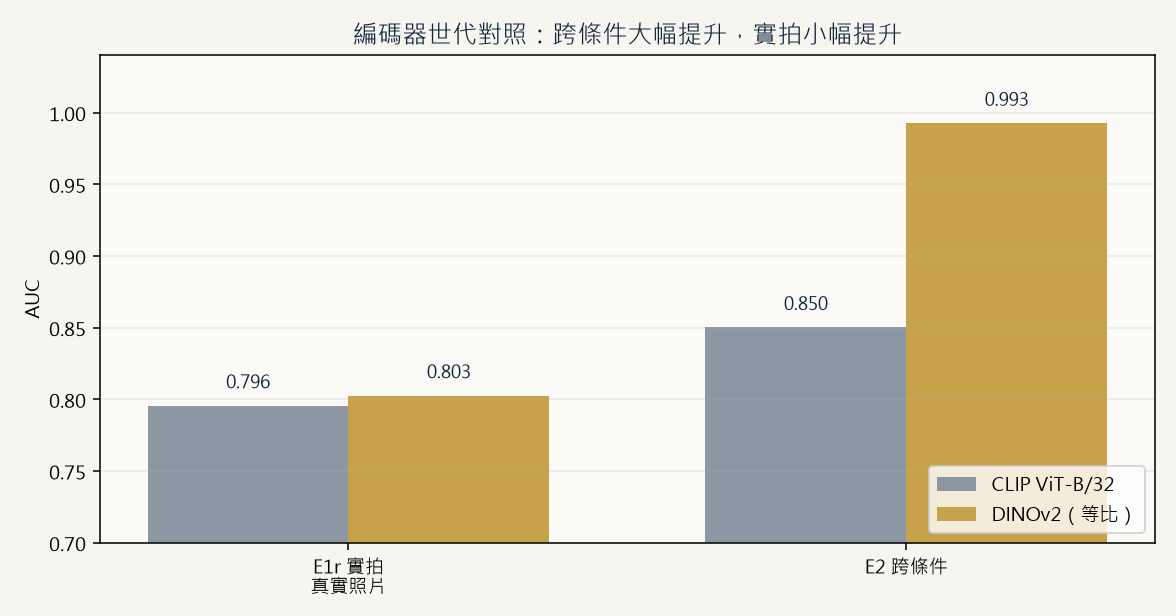
\includegraphics[width=0.82\linewidth]{figs/encoder-compare.png}
\caption{編碼器世代對照。跨條件（E2）提升最顯著，實拍（E1r）僅小幅提升——這正是「受控實驗不能推論真實世界」的直接證據。}\label{fig:enc}
\end{figure}

\begin{table}[H]
\centering
\small
\caption{編碼器對照（AUC）。E1 受控多視角、E1b 文物、E1r 公開實拍配對、E2 跨條件}
\begin{tabular}{lrrrrr}
\toprule
\textbf{設定} & \textbf{E1} & \textbf{E1b} & \textbf{E1r} & \textbf{E2} & \textbf{實拍最佳閾值} \\
\midrule
CLIP ViT-B/32（原基準） & 0.950 & 0.998 & 0.796 & 0.850 & 0.689 \\
DINOv2（壓成正方形） & 0.998 & 1.000 & 0.789 & 0.993 & 0.534 \\
\textbf{DINOv2（等比＋裁切）} & \hl{0.998} & 1.000 & \hl{0.803} & \hl{0.993} & \hl{0.193} \\
\bottomrule
\end{tabular}
\end{table}
\src{\texttt{docs/tech-evolution.tex} 階段 6；\texttt{tools/eval/out/report-dino-336cls.md}}

\begin{table}[H]
\centering
\small
\caption{編碼器世代的三個關鍵發現}
\begin{tabular}{p{1.0cm}p{14.2cm}}
\toprule
\textbf{發現} & \textbf{內容} \\
\midrule
(1) & \textbf{判別間距翻倍}：實拍的同棟／不同棟相似度差距由 0.138 擴大到 \hl{0.275}。間距比 AUC 更能反映「閾值穩不穩、能不能泛化到新資料」 \\
\addlinespace
(2) & \textbf{預處理比換模型更重要}：壓成正方形 0.789、等比縮放＋中心裁切 0.803。這個 0.014 的差距\textbf{比 CLIP 與 DINOv2 之間的差距還大} \\
\addlinespace
(3) & \textbf{產品閾值必須重新校準}：CLIP 最佳閾值 0.689，DINOv2 是 \hl{0.193}（DINOv2 餘弦值整體偏低）。原先產品使用的 0.86 對兩者都不適用 \\
\bottomrule
\end{tabular}
\end{table}

附帶發現：輸入邊長 336 px 與 518 px 的結果\textbf{完全相同}，池化方式（CLS 或 CLS+GeM）與翻轉增強的影響都在 0.002 以內——因此採用 336 px 以節省算力。\src{\texttt{tools/recognize/out/ablation-small336.json}}

\begin{table}[H]
\centering
\small
\caption{網站實際使用的編碼器設定（與歷史實驗不同，不可混用）}
\begin{tabular}{p{4.4cm}p{10.8cm}}
\toprule
\textbf{項目} & \textbf{設定} \\
\midrule
模型 & DINOv2 ViT-S/14（\texttt{facebook/dinov2-small}），384 維 \\
ONNX 檔案 & \texttt{public/models/dinov2-vits14-336.onnx}（87{,}186{,}817 bytes） \\
SHA-256 & \texttt{039dd80090cb7f6a2ff946cd5692b6594e8531405c29186085b774edd98809e2} \\
輸入 & 336 px，等比縮放最短邊 + 中心裁切 \\
TTA & 3 裁切（置中 + 左右各偏 12\%）× 水平翻轉，共 6 個視圖取平均後 L2 正規化 \\
池化 & CLS token，輸出已 L2 正規化 \\
推論 & onnxruntime-web（wasm），前端只算點積 \\
\bottomrule
\end{tabular}
\end{table}
\src{\texttt{public/data/memory-embeddings.json} 的 \texttt{encoder} 與 \texttt{preproc} 欄位；\texttt{tools/recognize/build\_embeddings.py}}

\qa{為什麼前端只算點積，而不是算完整餘弦相似度？}{因為所有向量（庫內與查詢端的）都已 L2 正規化，餘弦相似度等於點積：
\[ s(\mathbf{q},\mathbf{r}) = \frac{\mathbf{q}^{\top}\mathbf{r}}{\lVert\mathbf{q}\rVert_2 \lVert\mathbf{r}\rVert_2} = \mathbf{q}^{\top}\mathbf{r} \quad(\lVert\mathbf{q}\rVert=\lVert\mathbf{r}\rVert=1) \]
在瀏覽器裡，這省掉每一次比較的兩次開根號與兩次除法。更重要的是它\textbf{把「正規化」變成一個必須在兩端都成立的契約}：一旦前端載入的 ONNX 與建庫時用的不是同一個檔，查詢向量與庫內向量就落在不同分布——本專案真的發生過「同一張圖自相似度只有 0.06」，因此 \texttt{build\_embeddings.py} 會在輸出時直接比對兩個檔案的 SHA-256 並警告。}

\subsection{幾何驗證：不依賴 GPS 的第二道防線}

地理先驗能排除「外觀相近但距離很遠」的誤判，但\textbf{沒有 GPS 時就失效}（室內、地下、GPS 漂移）。幾何驗證提供不依賴位置的第二道防線：同棟不同角度會有大量\textbf{幾何一致}的特徵對應；不同棟即使整體相似，也難以找到一致的內點。

方法三步：全局檢索（DINOv2 餘弦相似度取 top-1 候選）→ 局部特徵（OpenCV SIFT，最多 2048 關鍵點，Lowe 比率檢驗 0.75）→ 幾何一致性（\texttt{cv2.findHomography} 搭配 USAC\_MAGSAC 穩健估計，統計內點數）。

\begin{figure}[H]
\centering
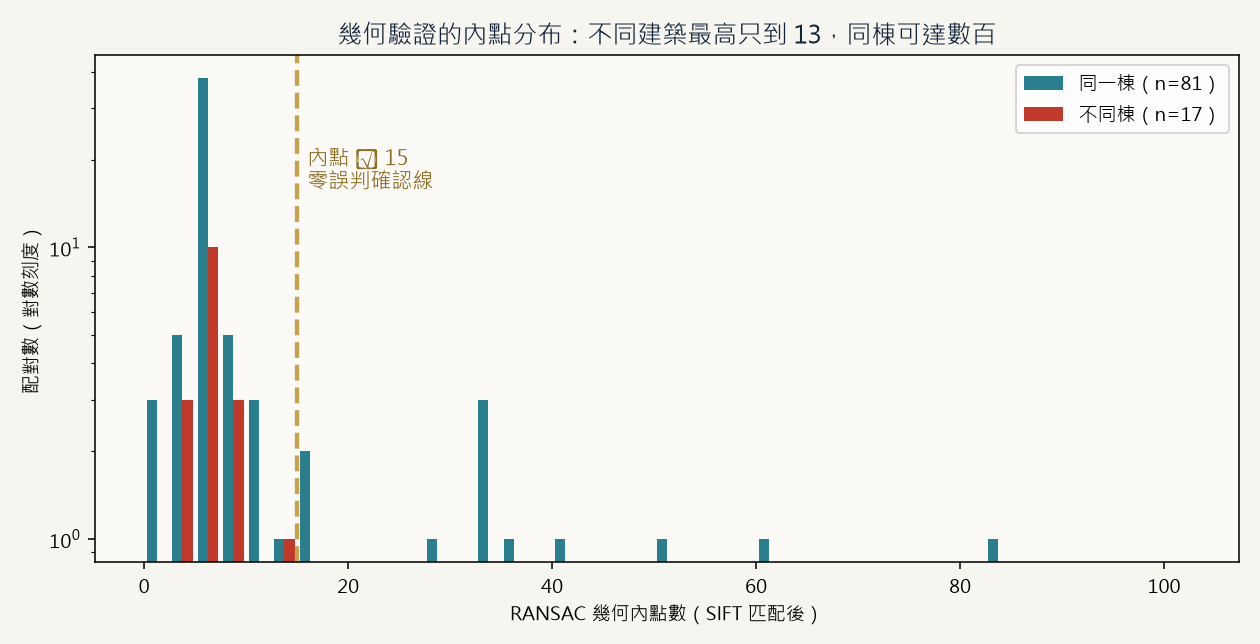
\includegraphics[width=0.80\linewidth]{figs/geo-inliers.png}
\caption{內點分布幾乎完全分離：不同建築最高只到 13 個內點，同棟可達數百。}
\end{figure}

\begin{table}[H]
\centering
\small
\caption{內點分布（98 對樣本：81 同棟、17 異棟）}
\begin{tabular}{lrrrr}
\toprule
\textbf{組別} & \textbf{中位內點} & \textbf{p90} & \textbf{最大} & \textbf{內點為 0 的比例} \\
\midrule
同一棟建築 & 7 & 501 & 2048 & 4\% \\
不同建築 & 6 & 8 & \warn{13} & 0\% \\
\bottomrule
\end{tabular}
\end{table}

\begin{table}[H]
\centering
\small
\caption{內點門檻掃描}
\begin{tabular}{lrrrr}
\toprule
\textbf{內點門檻} & \textbf{接受同棟} & \textbf{接受不同棟} & \textbf{精確率} & \textbf{召回} \\
\midrule
5 & 73 & 14 & 83.9\% & 90.1\% \\
10 & 30 & 1 & 96.8\% & 37.0\% \\
\textbf{15} & 26 & \hl{0} & \hl{100\%} & 32.1\% \\
20 & 24 & 0 & 100\% & 29.6\% \\
\bottomrule
\end{tabular}
\end{table}
\src{\texttt{tools/eval/geo\_verify.py}、\texttt{geo\_sweep.py}；\texttt{tools/eval/out/geo-verify-sift.json}}

\qa{內點 \ensuremath{\ge}15 時精確率 100\%，可以直接當成「同一棟」的判決嗎？}{可以，但\textbf{只能單向解讀}。這組有限樣本中接受 26 個正例、0 個負例，精確率的 Wilson 95\% 區間約 87.1\%\dash 100\%——有限樣本未觀察到誤接受，不保證新照片零誤判。}

\key{正確的用法是「確認器，不是過濾器」：}

\oneline{\textbf{內點 $\ge$ 15 $\Rightarrow$ 確定同一棟（此樣本 100\% 精確），可直接歸戶、不需 GPS；}\\[2pt]
\textbf{內點 $< $ 15 $\Rightarrow$ 退回全局相似度＋地理先驗，\warn{不可據此判為不同建築}。}}

原因是原理性的：\textbf{若兩張照片拍的是同一棟建築的不同立面，它們之間沒有共同的視覺內容，任何幾何方法都無法確認}——所以只能確認 32.1\% 的同棟配對。

\subsection{位置輔助排序：一個「故意做得很弱」的功能}

\begin{table}[H]
\centering
\small
\caption{位置輔助的設計約束（每一條都是刻意的限制）}
\begin{tabular}{p{4.2cm}p{11.0cm}}
\toprule
\textbf{設計} & \textbf{理由} \\
\midrule
每張照片預設關閉 & 位置只在使用者確認「這個位置對應目前照片」後才參與，避免把別處的 GPS 用到這張 \\
GPS 精度 $\le$ 100 m、採樣時間 $\le$ 5 分鐘 & 超過就退回純圖像，不讓過期或粗糙的位置影響排序 \\
距離降權最多 \hl{0.08} & 位置\textbf{不提高原始影像相似度}、不硬性排除遠景候選、不把接近候選自動升為高信心 \\
\warn{不自動消除視覺歧義} & 介面同頁比較「僅圖像」與「圖像＋位置」的首位候選，讓人看見位置到底改變了什麼 \\
\bottomrule
\end{tabular}
\end{table}
\src{\texttt{docs/location-upgrade.md}；\texttt{src/recognize/geo-ranking.js}；\texttt{docs/evidence-register.md}}

\qa{為什麼位置只降權 0.08，而不直接用它排除候選？}{因為位置資料本身也可能是錯的（室內、訊號遮蔽、使用者標錯建築輪廓）。若位置有權直接刪除候選，一次定位錯誤就會讓正確答案永遠不可能出現。相反地，\textbf{位置只做小幅降權，並把「僅圖像 vs 圖像＋位置」的差異顯示出來}，人就成為最後的仲裁者。這個決定讓功能的改善幅度看起來很小（改善幅度仍待獨立資料測量），但換來的是\textbf{不會因為一個錯誤的座標而靜默失敗}。}

\subsection{分類：小樣本時，任務不同就該用不同編碼器}

\begin{figure}[H]
\centering
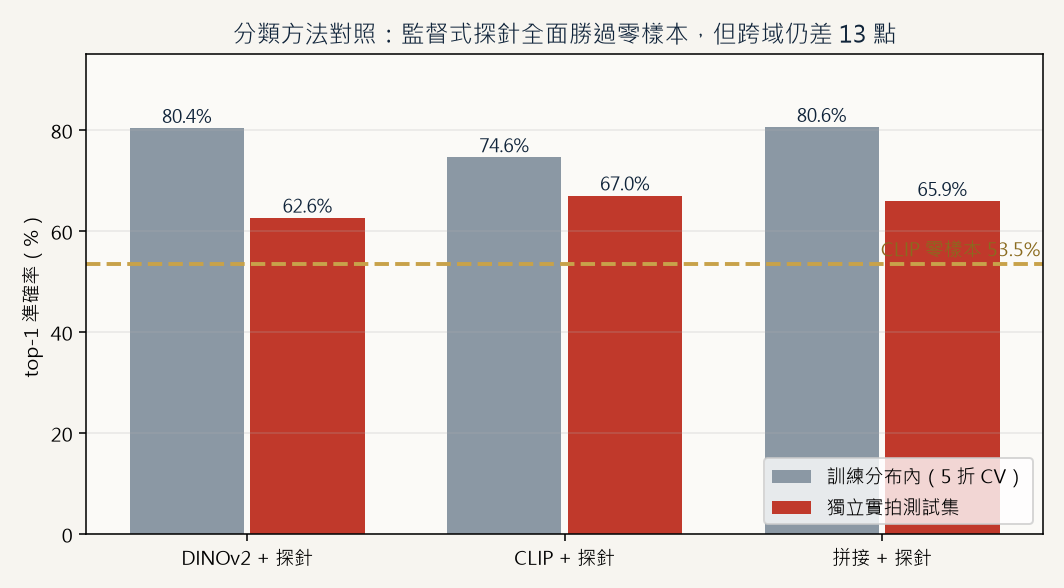
\includegraphics[width=0.78\linewidth]{figs/classifier-compare.png}
\caption{分類方法對照：凍結特徵 ＋ 線性探針全面勝過零樣本，但跨域仍有明顯落差。}
\end{figure}

\begin{table}[H]
\centering
\small
\caption{分類方法對照（11 類）}
\begin{tabular}{lrr}
\toprule
\textbf{方法} & \textbf{訓練分布內（5 折 CV）} & \textbf{獨立實拍測試集} \\
\midrule
CLIP 零樣本 & — & 53.5\% \\
\textbf{CLIP 特徵 ＋ 線性探針} & 74.6\% & \hl{67.0\%}（+13.5 點） \\
DINOv2 特徵 ＋ 線性探針 & \hl{80.4\%} & 62.6\% \\
拼接（CLIP ＋ DINOv2） & 80.6\% & 65.9\% \\
\bottomrule
\end{tabular}
\end{table}
\src{\texttt{tools/eval/probe\_classifier.py}；\texttt{docs/tech-evolution.tex} 階段 8}

\key{反直覺但重要的發現}：DINOv2 在訓練分布內更強（80.4\% vs 74.6\%），但 CLIP 特徵跨域泛化更好（67.0\% vs 62.6\%）——典型的小樣本域偏移現象，DINOv2 的細節特徵更容易過擬合訓練域。

\begin{center}
\begin{tikzpicture}
\node[draw=teal2,thick,fill=teal2!8,rounded corners,inner sep=8pt,text width=15.0cm,align=left] {
\textbf{\color{teal2}實務結論：任務不同就該用不同編碼器。}\\[3pt]
重辨識（同一棟不同角度）$\Rightarrow$ \textbf{DINOv2}（E2 +0.143，決定性優勢）\\
分類（小樣本、跨域）$\Rightarrow$ \textbf{CLIP 特徵 ＋ 線性探針}（67.0\%）};
\end{tikzpicture}
\end{center}

\subsection{「不修改模型架構」這個決定的意義}

值得強調的是：\textbf{本作品不修改任何模型架構}，而是以凍結特徵加上線性探針完成分類。這意味著效能的提升完全來自\textbf{資料品質與標註}，而非模型規模——這正好回到全文的主張：瓶頸在標註。而且凍結特徵在小樣本（數百張）下不易過擬合，是可重現、可稽核的做法。

%=====================================================================
\section{L5 品管與應用：從一筆紀錄到一座城市的檔案}

\subsection{編號：為什麼是 MM-YYYY-NNNN}

使用者要的語意很直接：\textbf{像貓臉辨識給每隻貓一個永久編號}，套在建築上——同一棟樓永遠同一個號，再拍一次要能自動認出併入。

\begin{table}[H]
\centering
\small
\caption{編號與建檔的欄位設計}
\begin{tabular}{p{4.0cm}p{11.2cm}}
\toprule
\textbf{欄位} & \textbf{作用} \\
\midrule
\texttt{code}（\texttt{MM-YYYY-NNNN}） & 唯一鍵；序號固定 4 位，超過 9999 自動變寬（\textbf{不截斷、不重號}） \\
\texttt{type} & YOLO 類別（11 類 + 街景），即「判定類型」的結果 \\
\texttt{lat}/\texttt{lng}、\texttt{accuracy\_m}、\texttt{sample\_count}、\texttt{geo\_source} & 座標與它的可信度；\texttt{geo\_source} 區分 \texttt{gps}/\texttt{wifi}/\texttt{manual}/\texttt{none} \\
\texttt{geo\_best\_accuracy\_m}、\texttt{geo\_spread\_m}、\texttt{geo\_stop\_reason} & 多次取樣的\textbf{過程}資訊，而不只是結果 \\
\texttt{location\_role}、\texttt{footprint\_id}、\texttt{capture\_location} & 區分「拍攝者位置」與「建築位置」；舊座標標為 \texttt{legacy-unverified} \\
\texttt{detector\_*}、\texttt{dedup\_*} & 這筆紀錄是由什麼辨識結果、什麼查重結論產生的 \\
\texttt{status} & \texttt{pending}/\texttt{approved}，保留人工複核入口 \\
\bottomrule
\end{tabular}
\end{table}
\src{\texttt{src/recognize/db.js} 的 \texttt{SCHEMA\_SQL}（\texttt{SCHEMA\_VERSION = 2}）}

\qa{為什麼要分開保存「拍攝者位置」與「建築位置」？}{因為這兩者在現場常常不是同一個點：使用者站在馬路對面拍，建築在 30 公尺外。若把 GPS 直接當成建築座標，整份檔案的空間精度會被拍攝位置綁死。因此系統要求使用者\textbf{主動在地圖上確認哪一棟是目標}（載入現有建築輪廓，放大後點選）；已確認建築位置時用建築位置，否則才用有效的裝置位置。未確認時，建築座標留空——\textbf{定位紀錄不代替建築座標}。}

\subsection{持久化：SQLite WASM + OPFS，以及三個「為什麼不是別的」}

\begin{table}[H]
\centering
\small
\caption{持久化方案的取捨}
\begin{tabular}{p{4.2cm}p{11.0cm}}
\toprule
\textbf{決策} & \textbf{理由} \\
\midrule
\warn{不用 \texttt{sql.js}} & 實測 \texttt{sql.js@1.14.2} 的 WASM \textbf{沒有編進 R-Tree}：\texttt{CREATE VIRTUAL TABLE ... USING rtree} 直接失敗（\texttt{no such module: rtree}）。而普查的核心需求就是 R-Tree 查重 \\
\key{用官方 \texttt{@sqlite.org/sqlite-wasm}} & \texttt{compile\_options} 內含 \texttt{ENABLE\_RTREE}（另有 FTS5／JSON／OPFS VFS）。R-Tree 是硬需求，因此選官方版 \\
WASM 在 Vite 的載入方式 & \texttt{import url from "@sqlite.org/sqlite-wasm/sqlite3.wasm?url"}，再交給 \texttt{initSqlite(\{ locateFile \})}；\textbf{不要放 \texttt{public/} 再 import}，也不要讓套件自己用 \texttt{import.meta.url} 猜（打包後會 404）。\texttt{vite.config.js} 的 \texttt{optimizeDeps.exclude} 必須含這個套件 \\
\bottomrule
\end{tabular}
\end{table}

持久化 provider 的選擇順序是 \textbf{OPFS → localStorage → memory}，並把「用了哪一種」回報到介面（\texttt{dbState().persistenceLabel}），讓使用者一眼看得出資料到底有沒有存下來。

\qa{為什麼不是「SQLite 直接長在 OPFS 上」？}{因為 OPFS VFS 的 \texttt{createSyncAccessHandle()} \textbf{只能在 Worker 裡呼叫}，而這個功能不需要那個複雜度：普查一次幾百到幾千筆，整庫匯出才幾百 KB。因此改用\textbf{非同步的 OPFS API}（\texttt{getFileHandle}/\texttt{createWritable}/\texttt{getFile}）在主執行緒操作。}

\qa{那高頻寫入與「來不及落地」怎麼辦？}{這是一個真實的失敗模式：非同步 OPFS 寫入有 350 ms 節流，如果使用者在節流窗內就按了重新整理，寫入可能來不及完成。解法是\textbf{當 OPFS 是主 provider 時，同步再寫一份位元組快照到 localStorage}（\texttt{setItem} 是同步 API，關頁時一定寫得完）；下次開啟時兩份比時間戳，取新的。localStorage 當主 provider 時本身就是同步寫入，不需要快照。}

\subsection{R-Tree 空間查重：為什麼是兩段式}

\begin{equation}
\text{R-Tree 粗篩（bbox）} \;\longrightarrow\; \text{haversine 精算} \;\longrightarrow\; \text{候選清單給人核對}
\end{equation}

\begin{center}
\begin{tikzpicture}
\node[draw=red2!60,thick,fill=red2!6,rounded corners,inner sep=7pt,text width=15.0cm,align=left] {
\textbf{為什麼不能只用 R-Tree：}SQLite 的 rtree 座標欄位是 \textbf{32 位元浮點}，在澳門的經度（113.54 附近）解析度\textbf{約 1 公尺}。因此 R-Tree 只當「便宜的粗篩」（查詢框多留 2 公尺安全邊際），精確距離一律用 \texttt{REAL} 欄位的原始座標算 haversine 再過濾。};
\end{tikzpicture}
\end{center}
\src{\texttt{src/recognize/geo-math.js} 的 \texttt{bboxForRadius()}；\texttt{db.js} 的 \texttt{findNearby()}}

\subsection{GPS 多次取樣：加權平滑，但不假裝變準}

\begin{table}[H]
\centering
\small
\caption{三種取樣計畫}
\begin{tabular}{lrrl}
\toprule
\textbf{計畫} & \textbf{最多樣本} & \textbf{間隔} & \textbf{目標估計範圍} \\
\midrule
快速 & 8 & 250 ms & $\le 15$ m \\
標準（預設） & 30 & 1000 ms & $\le 5$ m \\
延長取樣 & 40 & 1000 ms & $\le 3$ m \\
\bottomrule
\end{tabular}
\end{table}

座標以 $1/\text{accuracy}^2$ 加權平均：

\begin{equation}
\hat{\mathbf{p}} = \frac{\sum_i w_i \mathbf{p}_i}{\sum_i w_i}, \qquad w_i = \frac{1}{a_i^{2}}
\end{equation}

\begin{table}[H]
\centering
\small
\caption{兩種現場失敗情境，以及系統的處理方式}
\begin{tabular}{p{3.6cm}p{2.6cm}p{8.8cm}}
\toprule
\textbf{情境} & \textbf{判據} & \textbf{處理} \\
\midrule
裝置可能沒有 GPS 晶片（筆電常見） & 估計範圍 $>30$ m & 明確顯示「此裝置可能沒有 GPS 晶片」，並\textbf{自動展開手動定位}（直接載入建築輪廓讓人對位） \\
讀數跳動過大 & 樣本離散 $>50$ m & 顯示「讀數跳動過大」 \\
\bottomrule
\end{tabular}
\end{table}

\begin{center}
\begin{tikzpicture}
\node[draw=gold,very thick,fill=gold!12,rounded corners,inner sep=8pt,text width=15.0cm,align=left] {
\textbf{最重要的設計決定：最終精度是保守的。}\\[3pt]
讀數完全一致時就回報最佳單次精度，\warn{不除以 $\sqrt{n}$ 假裝變準}；估計圈也不隨樣本數縮小。\\
手動座標標記為 \texttt{geo\_source='manual'}、\texttt{accuracy\_m=NULL}，原 GPS 讀數留在 \texttt{geo\_note}。};
\end{tikzpicture}
\end{center}

\qa{為什麼不做 $\sqrt{n}$ 縮小？}{因為瀏覽器的 \texttt{accuracy} 是設備回報的水平誤差半徑（規格要求 95\% 信心水準），而\textbf{連續讀數之間有相關性}——同一個錯誤的衛星幾何會讓連續 30 次讀數一起偏。把它們當成 30 個獨立觀測來縮小誤差，會得到一個看起來很漂亮但沒有依據的精度值。寧可回報「最佳單次精度」，讓使用者自己判斷要不要手動對位。\src{\texttt{src/recognize/geo-math.js}；\texttt{docs/location-upgrade.md}}}

\subsection{為什麼第一階段不做 OPFS 持久化}

\begin{quote}
\textbf{第一階段：資料庫在記憶體，靠匯出 \texttt{.sqlite}／JSON 保存}（每筆同時鏡射到 localStorage 的 \texttt{macau-memory.pending-discoveries}）。持久化介面已預留：\texttt{openDb(\{ persistence \})} 換一個有三個非同步方法的 adapter 即可，其餘程式碼不用動。
\end{quote}

\warn{這是歷史記錄，現況已經改變}：目前的 \texttt{db.js} 已實作 \texttt{opfsPersistence}（含可用性探測、毀損隔離 \texttt{.corrupt-<時間戳>}、localStorage 同步快照備援），並在 \texttt{openDb()} 中依 OPFS → localStorage → memory 自動挑選。此處保留第一階段的決策紀錄，是因為\textbf{介面先行的作法本身就是一個值得講解的決定}：先把 persistence 抽成介面再延後實作，使得後續加入 OPFS 不需要改動呼叫端。

%=====================================================================
\section{關鍵數據與證據}

\subsection{一張表看懂：哪些數字可以一起講，哪些不行}

\src{本節口徑依 \texttt{docs/evidence-register.md}（更新 2026-09-30）：報告、簡報與影片應區分受控渲染、公開照片配對、參考庫留一法和獨立實拍；\textbf{不同任務的 AUC、Top-1、mAP 不能互換}。}

\begin{table}[H]
\centering
\small
\caption{成果與證據口徑總表}
\begin{tabular}{@{}p{2.6cm}p{4.0cm}p{4.0cm}>{\raggedright\arraybackslash}p{4.2cm}@{}}
\toprule
\textbf{成果} & \textbf{可核對的結果} & \textbf{範圍與限制} & \textbf{證據} \\
\midrule
網頁 DINOv2 檢索 & 38 棟／335 張；LOO Top-1 \hl{88.96\%}、Top-3 \hl{94.93\%} & 查詢自參考庫留出一張，其餘同棟照片保留；\warn{未隔離攝影者與拍攝批次}，不是獨立遊客準確率 & \pth{memory-embeddings.json} 的 \pth{eval}；\pth{build_embeddings.py} \\
\addlinespace
歷史 DINOv2-base 受控配對 & E1 AUC 0.998；E2 AUC 0.993 & E2 是 GLB 改變光照／角度／距離的\textbf{渲染}；不是跨日期實拍。編碼器為 base@336，與網頁 small ONNX 不同 & \pth{tools/eval/out/metrics-dino-336cls.json} \\
\addlinespace
歷史公開實拍配對 & E1r AUC 約 0.803 & 配對分類指標；不可替代網頁端到端辨識率 & 同上 E1r \\
\addlinespace
離線 SIFT + RANSAC & 98 對：81 同棟、17 異棟；接受 26 正例、0 負例；正例接受率 26/81 = 32.1\% & 精確率 26/26 是有限樣本的觀測值；Wilson 95\% 約 87.1\%\dash 100\%，\warn{不是「永不誤判」}；未接入網頁辨識流程 & \pth{tools/eval/out/geo-verify-sift.json} \\
\addlinespace
位置輔助排序 & 已接入；每張照片預設關閉；GPS $\le$100 m、$\le$5 分鐘；距離降權最多 0.08 & 不提高原始影像相似度、不硬性排除遠景、不把接近候選自動升為高信心；\warn{改善幅度待獨立資料測量} & \pth{src/recognize/geo-ranking.js} \\
\addlinespace
地圖精細模型替換 & 四個約 190 萬面模型；14 級預覽、16.5 級按視野載入 & \warn{AI 生成且非實測尺度}；展示尺寸／朝向／定位暫定，沒有測繪精度結論 & \pth{docs/high-precision-glb.md} \\
\addlinespace
獨立實拍驗收 & 工具與防洩漏檢查已完成；\warn{指標待採集} & 必須填來源、攝影者、批次與拍攝日期，攝影者／批次隔離，SHA-256 查重 & \pth{tools/recognize/independent-eval.mjs} \\
\addlinespace
位姿投影標註／上軸推估 & \warn{研究與整合方向} & 本倉庫的預標註入口是 YOLO-World；外部桌面重建模組的專案數與測試數尚缺可核對清單與日誌 & \pth{tools/yolo-dataset/prelabel.py} \\
\bottomrule
\end{tabular}
\end{table}

\subsection{必須處理的矛盾：335 張 88.96\% 對上 322 張 89.1\%}
\label{sec:conflict}

專案內存在\textbf{兩組互相矛盾的辨識數據}。我們沒有選一組假裝沒問題，而是先查證。

\begin{table}[H]
\centering
\small
\caption{矛盾的兩組數字}
\begin{tabular}{p{4.6cm}rrr}
\toprule
\textbf{來源} & \textbf{參考影像數} & \textbf{Top-1} & \textbf{Top-3} \\
\midrule
對外敘述（\texttt{README.md} / 影片 / 競賽報告 / 專案報告） & \textbf{335} & \textbf{89.0\%}（88.96\%） & \textbf{94.9\%}（94.93\%） \\
\texttt{docs/figs/recognize-all-summary.png} 圖上標示 & \textbf{322} & \textbf{89.1\%} & \textbf{95.7\%} \\
\bottomrule
\end{tabular}
\end{table}

\key{查證方法與結果}：直接讀取 \texttt{public/data/memory-embeddings.json}，並以獨立腳本重算留一法（不信任檔案內已存的 \texttt{eval} 欄位），得到：

\begin{verbatim}
=== 獨立重算 public/data/memory-embeddings.json 的留一法 ===
generated        : 2026-09-26T22:19:07
encoder          : DINOv2 ViT-S/14 (facebook/dinov2-small) | dim 384
buildings        : 38
reference images : 335          <-- 實際在庫的參考向量總數
n_queries scored : 335
Top-1            : 298/335 = 0.8896 (88.96%)
Top-3            : 318/335 = 0.9493 (94.93%)
stored eval field: {"n_queries": 335, "n_buildings": 38,
                    "top1": 0.8896, "top3": 0.9493, ...}
\end{verbatim}

\key{差異來源（已定位）}：\texttt{docs/figs/recognize-all-summary.png} 是 \texttt{tools/recognize/visualize\_all.py} 產生的圖，該腳本的標題直接寫入「\texttt{f"留一法辨識準確率（\{n\} 張參考照片）"}，其中 \texttt{n} 是\textbf{執行當下}庫內的向量總數。因此 \textbf{322 是一次較早的評測跑出來的圖}：那時庫內是 322 條向量（38 棟、無 6 張模型截圖），之後擴充參考庫才變成 335 條。同一件事在倉庫的影片計畫檔中已有獨立記錄：\texttt{plans/macau-memory-web-3min.plan.md} 第 7 節明確指出該圖是\textbf{較舊的一次評測}，並記錄真站讀出的 \texttt{libMeta.eval} 為 \texttt{n\_queries: 335, top1: 0.8896, top3: 0.9493}，因此該影片\textbf{刻意不使用那張舊圖}。

\oneline{\textbf{本文採用的數字：38 棟 / \hl{335} 張參考照片 / Top-1 \hl{88.96\%} / Top-3 \hl{94.93\%}。}\\[3pt]
{\small 依據：獨立重算結果與檔案內 \texttt{eval} 欄位一致；且 335 = 329 張實拍 + 6 張本站模型截圖，可與 \texttt{build\_embeddings.py} 的收錄規則逐項對上。}}

\warn{這組數字仍然不是「真實世界準確率」}：此實驗的查詢是從參考庫留出一張，\textbf{沒有隔離攝影者與拍攝批次}。同一棟的 5 張照片可能來自同一位攝影者的同一天，因此比「真實世界陌生人隨手拍」樂觀。獨立實拍評測的工具與防洩漏檢查已完成，但指標待採集。

\subsection{檢索表現的可信區間（超幾何分布的精確區間）}

Top-1 = 298/335 是一個比例估計，應附上不確定性。以 Clopper\dash Pearson（Beta）精確區間計算：

\begin{table}[H]
\centering
\small
\caption{留一法指標的點估計與 95\% 精確區間}
\begin{tabular}{lrrr}
\toprule
\textbf{指標} & \textbf{命中／總數} & \textbf{點估計} & \textbf{95\% 精確區間} \\
\midrule
Top-1 & 298 / 335 & 88.96\% & 85.10\%\dash 92.10\% \\
Top-3 & 318 / 335 & 94.93\% & 91.98\%\dash 97.02\% \\
\bottomrule
\end{tabular}
\end{table}

\src{由本文以 \texttt{scipy.stats.beta} 依 298/335 與 318/335 計算；方法與 \texttt{geo-verify-sift.json} 使用的 Wilson 區間屬同一類「比例區間」概念}

\subsection{逐棟表現：哪些建築會被認錯}

\begin{table}[H]
\centering
\small
\caption{參考庫的逐棟參考張數（節錄；完整 38 棟見 \texttt{memory-embeddings.json}）}
\begin{tabular}{lr@{\hspace{8mm}}lr}
\toprule
\textbf{建築} & \textbf{參考張數} & \textbf{建築} & \textbf{參考張數} \\
\midrule
澳門旅遊塔 & 17 & 龍環葡韻住宅式博物館 & 14 \\
大三巴牌坊 & 17 & 媽閣廟 & 13 \\
葡京酒店（新葡京） & 13 & 港務局大樓 & 13 \\
玫瑰堂（聖多明我教堂） & 13 & 鄭家大屋 & 12 \\
民政總署大樓 & 11 & 崗頂劇院 & 10 \\
澳門銀河 & 10 & 東望洋炮台及燈塔 & 10 \\
觀音蓮花苑 & 10 & 盧家大屋（金玉堂） & 10 \\
澳門科學館 & 10 & 澳門巴黎人 & 10 \\
聖若瑟修院及聖堂 & 10 & 澳門威尼斯人 & 10 \\
\addlinespace
路環市區 & 5 & 氹仔舊城區 & 5 \\
觀音堂（普濟禪院） & 5 & 紅街市（提督街市） & 5 \\
福隆新街 & 5 & 澳門漁人碼頭 & 4 \\
荔枝碗船廠 & 4 & 議事亭前地 & 4 \\
主教座堂（大堂） & \warn{3} & 澳門大賽車博物館 & \warn{3} \\
澳門博物館 & \warn{3} & & \\
\bottomrule
\end{tabular}
\end{table}
\src{逐棟 \texttt{count} 欄位。\warn{注意}：參考張數少的建築（3\dash 5 張）在留一法下等於只有 2\dash 4 個同棟鄰居可用，其單棟準確率的統計不確定性遠大於參考張數多的建築。}

\begin{figure}[H]
\centering
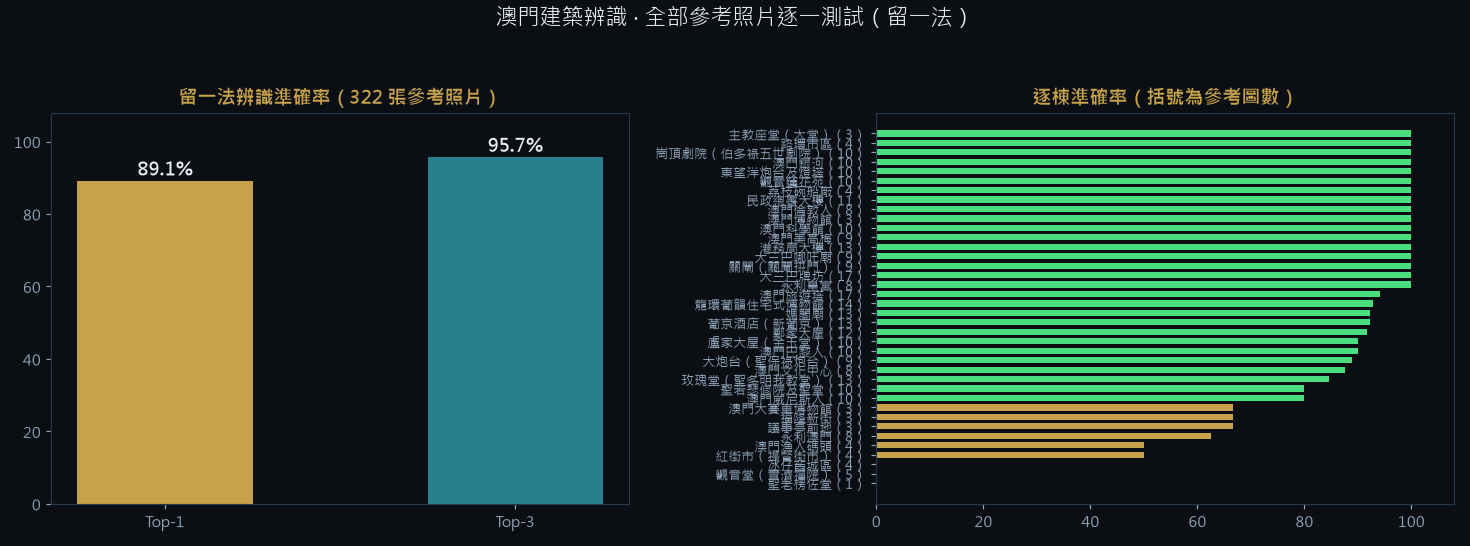
\includegraphics[width=\linewidth]{figs/recognize-all-summary.png}
\caption{\warn{注意：本圖上的「322 張參考照片 / Top-1 89.1\% / Top-3 95.7\%」是較早一次評測的數字}，與本文採用的 335 張 / 88.96\% / 94.93\% 不同，差異來源見 §\ref{sec:conflict}。保留本圖是為了讓讀者能自行核對這組矛盾，而不是把它當成現行指標。}
\end{figure}

\begin{figure}[H]
\centering
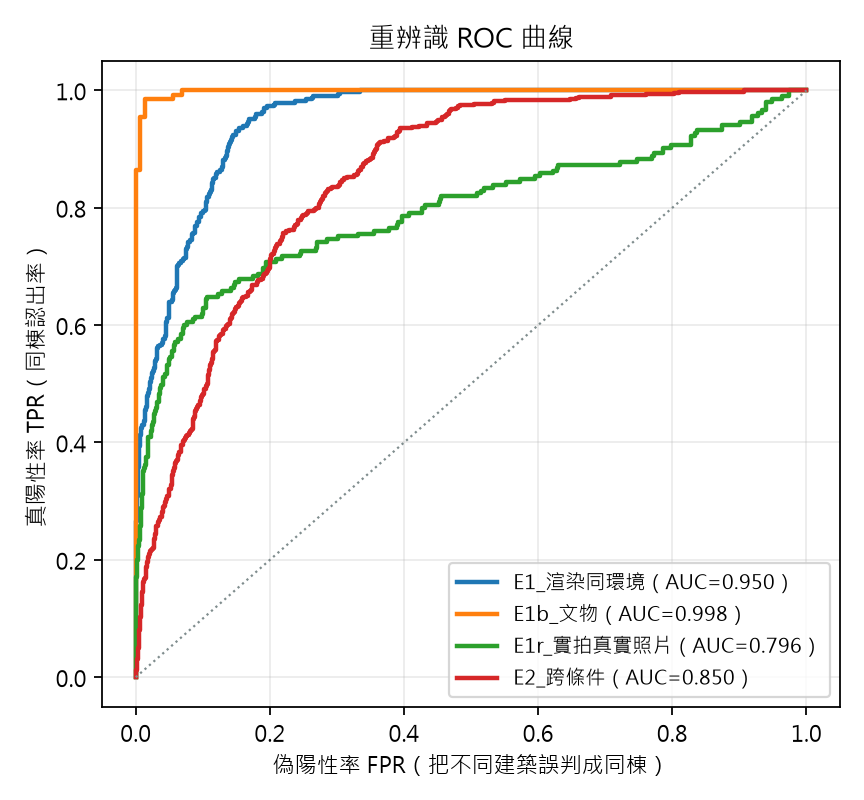
\includegraphics[width=0.86\linewidth]{figs/roc.png}
\caption{配對判別的 ROC 曲線。\warn{本圖是 CLIP 世代}：四條曲線分別為 E1 受控多視角（AUC 0.950）、E1b 文物（0.998）、E1r 公開實拍（0.796）、E2 跨條件（0.850）。DINOv2 世代的 E2 提升至 0.993（見圖 \ref{fig:enc}）。AUC 高不代表端到端準確率高——查詢條件、資料範圍與任務定義都不同。}
\end{figure}

\begin{figure}[H]
\centering
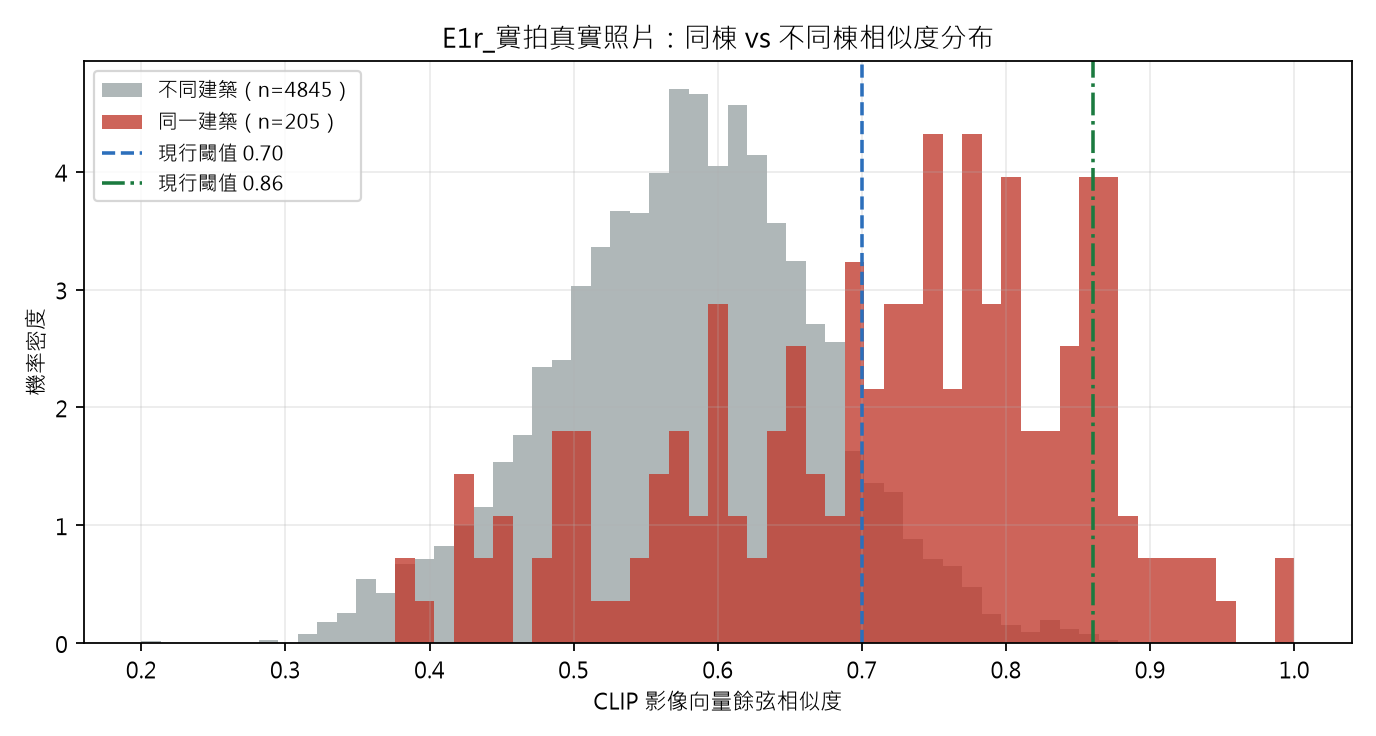
\includegraphics[width=0.62\linewidth]{figs/hist-real.png}
\caption{E1r 公開實拍配對的相似度分布（CLIP 世代，205 組正樣本 / 4{,}845 組負樣本）：同棟與不同棟\textbf{大量重疊}。圖上兩條垂直線是當時的產品門檻 0.70 與 0.86——0.86 在渲染圖上可認出 86.1\%，套到真實照片只剩 14.1\%。這是「實拍比渲染難」最直接的圖像證據，也是為什麼必須引入位置先驗與幾何驗證。}
\end{figure}

\subsection{端到端偵測：YOLO 在沒見過的照片上}

\begin{table}[H]
\centering
\small
\caption{在 49 張未見真實照片上的檢測表現}
\begin{tabular}{lcc}
\toprule
\textbf{指標} & \textbf{基線} & \textbf{本作品} \\
\midrule
成功檢測出建築 & 57\% & \hl{65\%} \\
檢測且類別正確 & 43\% & \hl{56\%} \\
\bottomrule
\end{tabular}
\end{table}
\src{\texttt{tools/yolo-dataset/eval\_on\_cc.py}；\texttt{docs/tech-evolution.tex} 階段 4}

\begin{figure}[H]
\centering
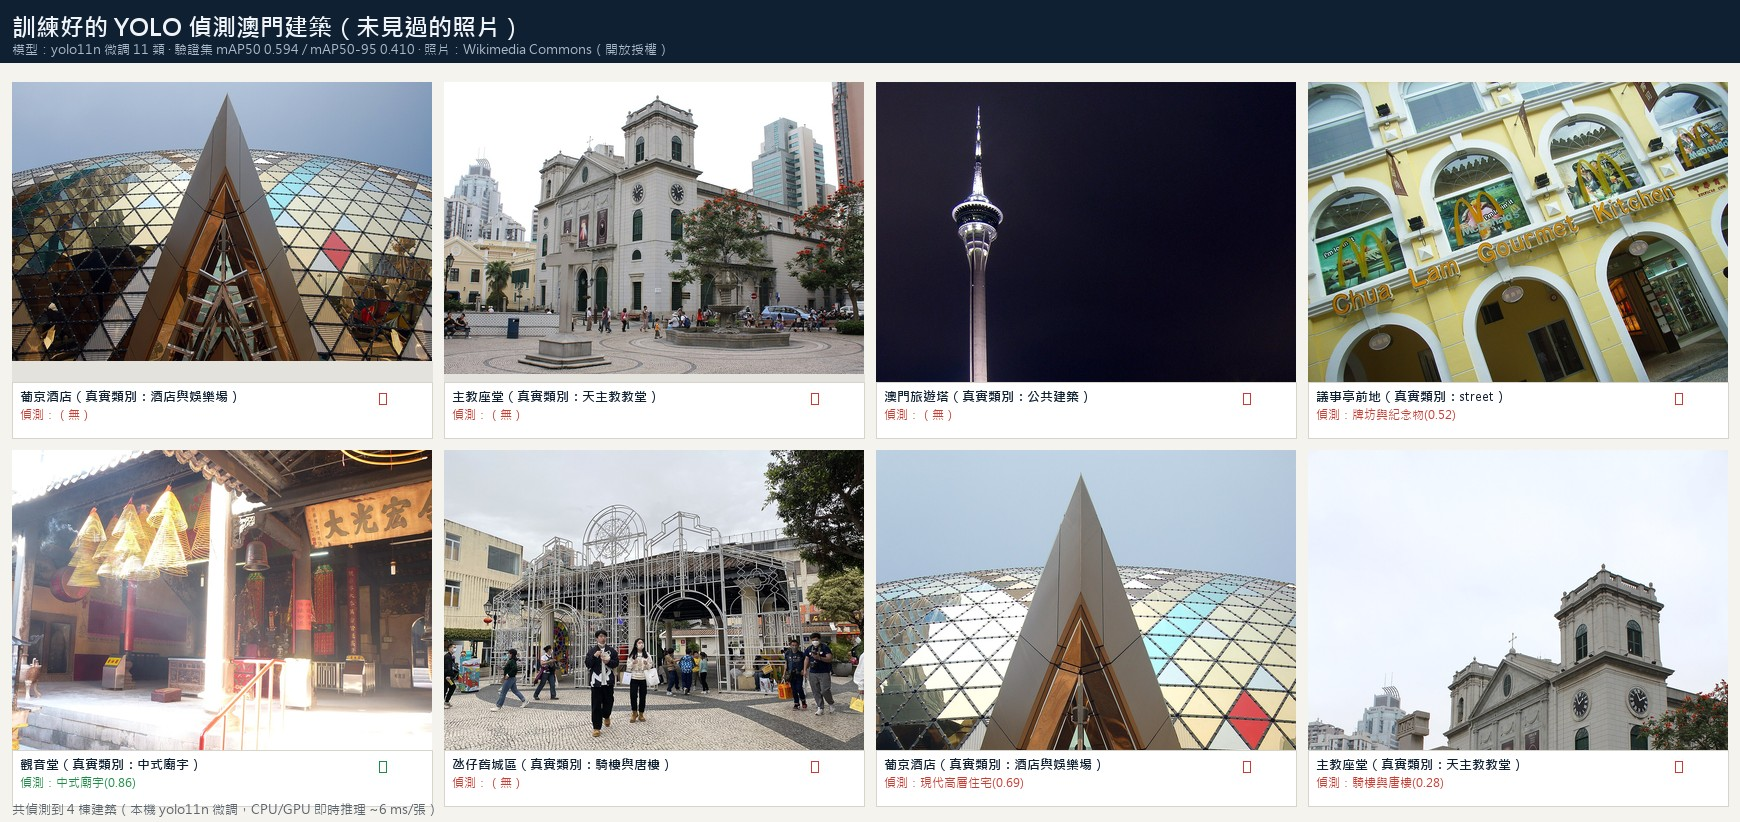
\includegraphics[width=\linewidth]{figs/detect-demo.jpg}
\caption{偵測結果示例。類別標籤來自 11 類自訓模型；框的鬆緊程度反映了「弱標註」的血統——這些框由 YOLO-World 產生，人工尚未逐張修正。}
\end{figure}

\begin{figure}[H]
\centering
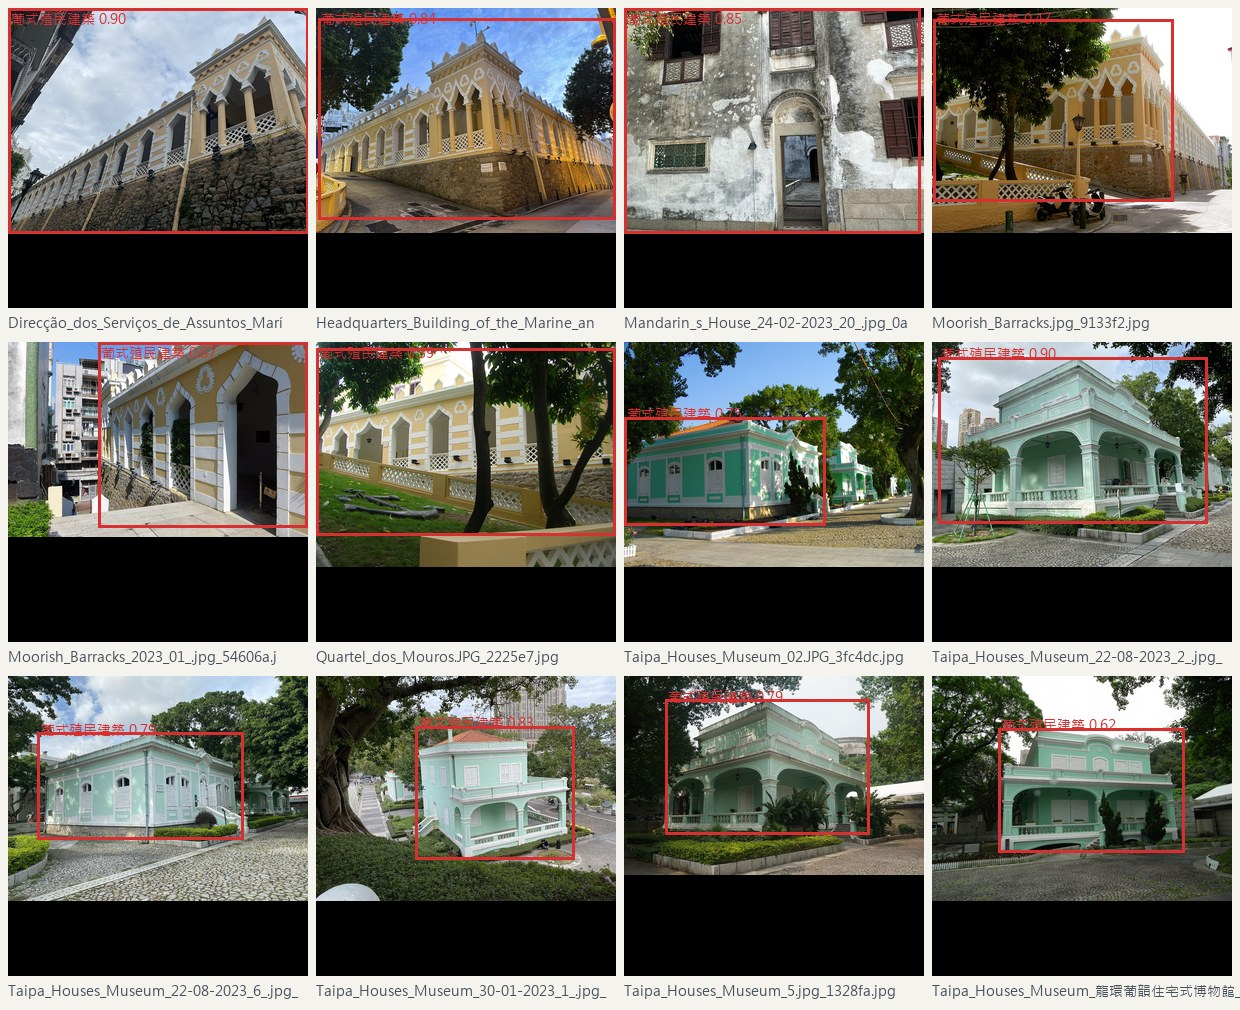
\includegraphics[width=0.86\linewidth]{figs/prelabel.jpg}
\caption{自動預標註的介面。標註管線的設計目標不是「一次到位」，而是「把人工從畫框降級為修框」。}
\end{figure}

\subsection{為什麼路氹城三棟度假村是整個系統的試金石}

\begin{table}[H]
\centering
\small
\caption{視覺誤判 100\% 集中在路氹城三棟外觀相近的度假村}
\begin{tabular}{lrr}
\toprule
\textbf{建築配對} & \textbf{平均相似度} & \textbf{相似度 $>0.86$ 的比例} \\
\midrule
澳門倫敦人 vs 澳門銀河 & 0.874 & \warn{72.2\%} \\
澳門巴黎人 vs 澳門銀河 & 0.840 & 31.2\% \\
澳門倫敦人 vs 澳門巴黎人 & 0.826 & 18.8\% \\
其餘 7 組配對 & 0.70\dash 0.75 & \ok{0.0\%} \\
\bottomrule
\end{tabular}
\end{table}

關鍵事實：這三棟建築兩兩相距 \textbf{至少 296 公尺}（中位數 4{,}302 公尺）。以 90 公尺為半徑的地理先驗，可直接排除全部誤判候選。

\oneline{\textbf{視覺比對只負責「同一棟的不同角度」；地理先驗負責「不可能是我」。}\\[3pt]
{\small 這個分工是後續所有設計的基礎：視覺模型不需要（也不可能）做到完美。}}

\begin{figure}[H]
\centering
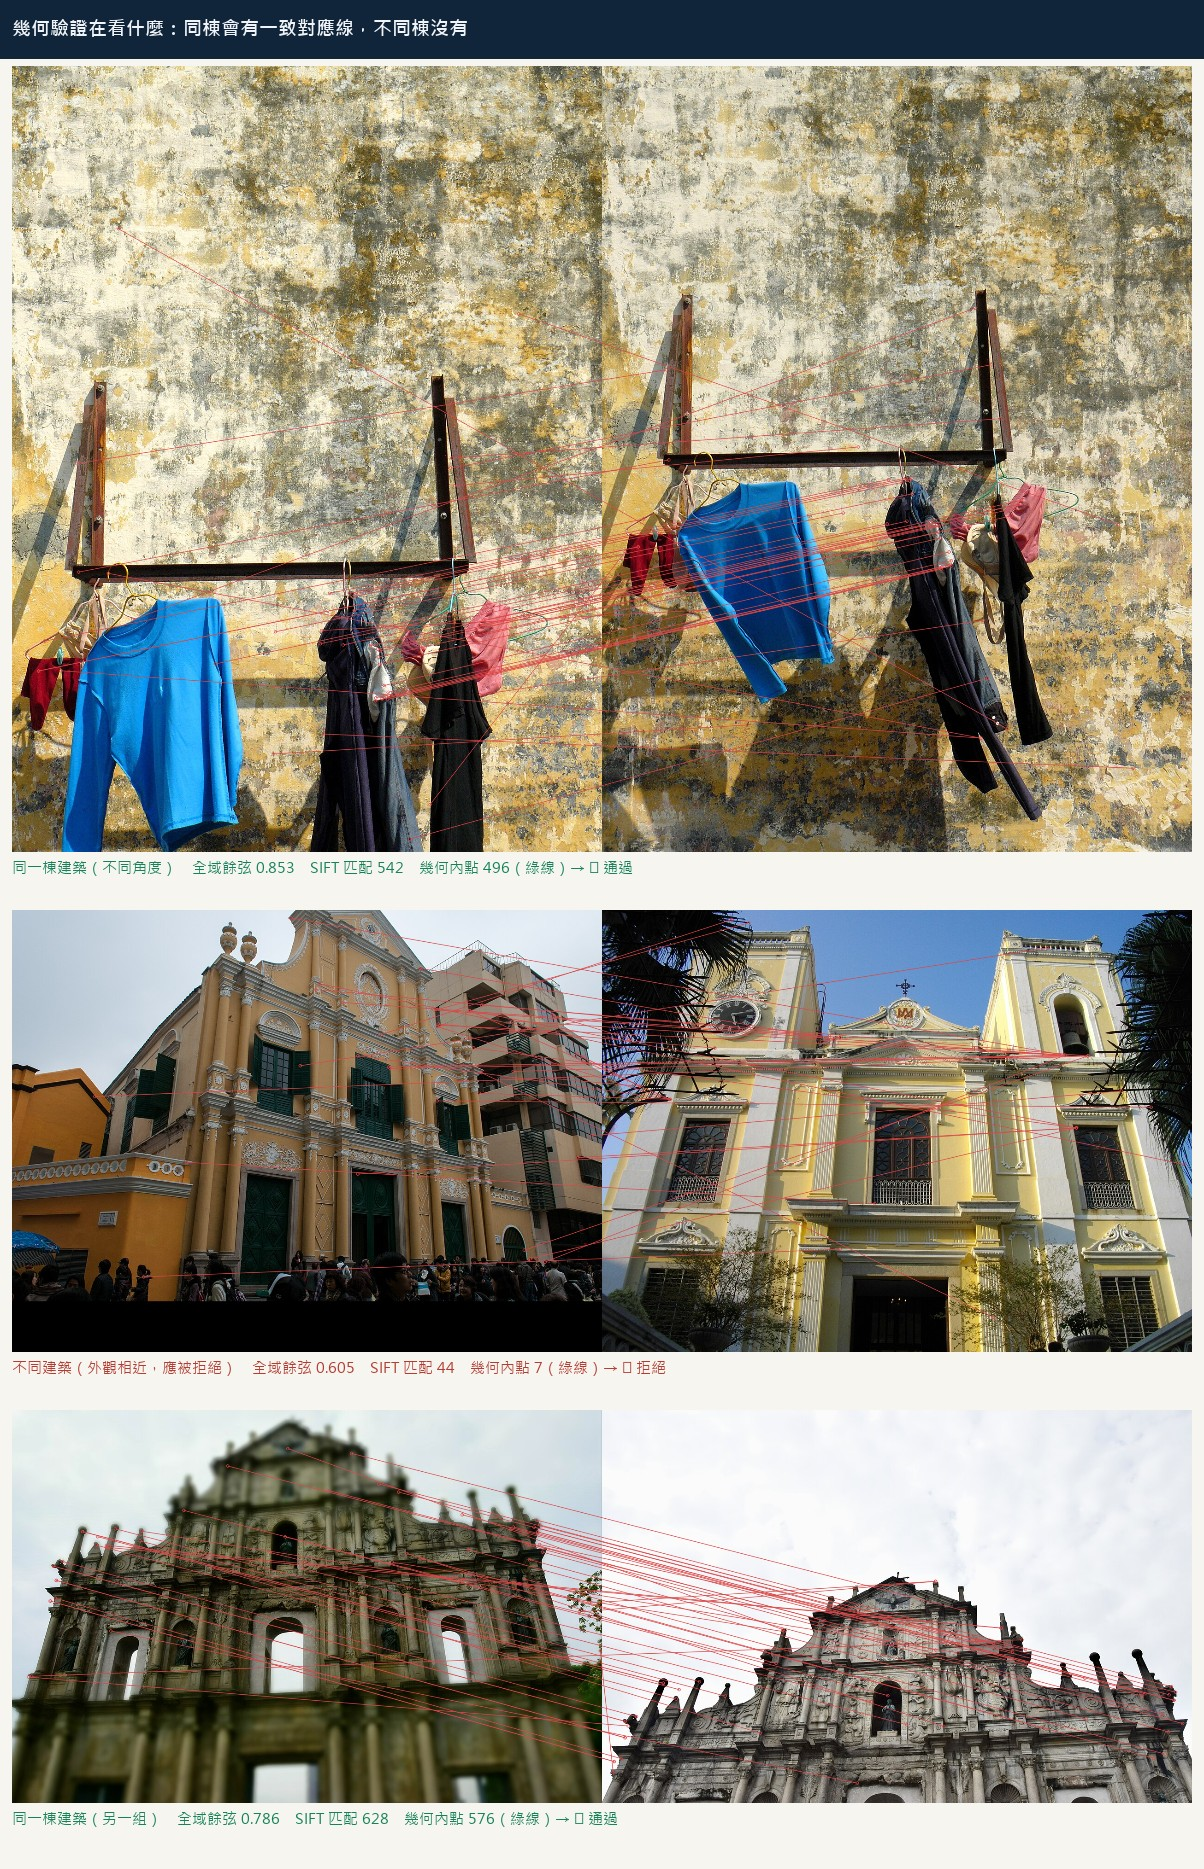
\includegraphics[width=\linewidth]{figs/demo-geo-verify.jpg}
\caption{位置確認與地理驗證的實際介面流程：拍攝者位置與建築位置分開保存，使用者必須主動確認「這個位置對應目前照片」。}
\end{figure}

%=====================================================================
\section{技術棧與實作}

\subsection{網站端：vanilla JS + MapLibre GL + DEM + ONNX Runtime Web}

\begin{table}[H]
\centering
\small
\caption{網站端技術棧（\texttt{package.json} 實測版本）}
\begin{tabular}{p{4.4cm}rp{9.0cm}}
\toprule
\textbf{元件} & \textbf{版本} & \textbf{承擔的職責} \\
\midrule
Vite & \textasciitilde 8.3 & 建置與開發伺服器；WASM 資產路徑處理 \\
MapLibre GL JS & \textasciitilde 6.10 & 地理資料渲染、地形（DEM）、圖層管理 \\
three.js & \textasciitilde 0.186 & GLB 模型檢視、導航動畫 \\
PlayCanvas & 2.21.4 & 3DGS 高斯實景渲染（優先 WebGPU，回退 WebGL2） \\
\texttt{@sqlite.org/sqlite-wasm} & \textasciitilde 3.53.4 & 本機結構化檔案管理、R-Tree 空間查詢 \\
geotiff & \textasciitilde 3.0 & DEM 高程資料讀取 \\
ONNX Runtime Web & （隨頁載入） & 瀏覽器端 YOLO 與 DINOv2 推論（wasm） \\
OpenCC-JS & \textasciitilde 1.4 & 繁簡轉換（跨端資料顯示） \\
\bottomrule
\end{tabular}
\end{table}

\begin{table}[H]
\centering
\small
\caption{端側模型規格}
\begin{tabular}{p{4.0cm}rp{8.4cm}}
\toprule
\textbf{模型} & \textbf{檔案大小} & \textbf{設定} \\
\midrule
YOLO11s 澳門建築 11 類 & 38.0 MB & \texttt{imgsz=768}、opset 17、類別感知 NMS 在前端 \\
DINOv2 ViT-S/14 & 87.2 MB & 336 px、3 裁切 × 翻轉、CLS pooling、384 維、已 L2 正規化 \\
DINOv2（int8 量化） & 23.0 MB & 供低頻寬環境使用（與上列為不同檔案） \\
\bottomrule
\end{tabular}
\end{table}

\qa{為什麼模型不放伺服器？}{兩個理由。第一，\textbf{隱私}：照片不離開裝置，也就不需要處理上傳的同意、保存與刪除。第二，\textbf{可用性}：普查現場常在戶外、訊號不穩，端側推論不受網路影響。代價是首次載入要下載 125 MB 的模型（YOLO 38 MB + DINOv2 87 MB），因此介面上必須讓使用者看到載入進度，而不是空白等待。}

\subsection{桌面端：Tauri 2 + Rust + React 19}

重建與標註在桌面端（MacauSplat）執行，核心引擎以 Rust 實作，前端為 React 19；全部影像與三維處理在本機完成，不上傳雲端。

\begin{table}[H]
\centering
\small
\caption{工程驗證（標註模組的測試覆蓋）}
\begin{tabular}{lrl}
\toprule
\textbf{項目} & \textbf{數量} & \textbf{說明} \\
\midrule
後端單元測試 & \hl{190} & 含二進位格式往返、投影幾何、上軸推定、包圍盒擬合、離群修剪、品質判定 \\
前端單元測試 & \hl{137} & 含三維投影數學、點雲繪製、輪詢生命週期 \\
靜態檢查 & 0 警告 & 格式化與靜態分析全數通過 \\
真實專案驗證 & \hl{8} & 端到端跑通，其中 3 個因相機註冊率過低被正確判為不可用 \\
\bottomrule
\end{tabular}
\end{table}

\warn{證據邊界（必須明講）}：上表的 190／137／8 出自早期的競賽報告，而 \texttt{docs/evidence-register.md} 明確記載「舊報告中的外部桌面重建模組、8 個專案與 327 項測試尚缺可核對的程式、資料清單、日誌；不得列為本網站已驗證成果」。本倉庫\textbf{確實存在}可讀的 Rust 原始碼（\texttt{tools/integration/splat/*.rs}、\texttt{output/integration/splat-edits/src-tauri/src/reconstruction/*.rs}）與其內嵌的 \texttt{\#[test]} 案例，但本文\textbf{未執行} \texttt{cargo test}，因此不把這些數字列為本次查核通過的成果。

\begin{table}[H]
\centering
\small
\caption{標註模組內部可見的單元測試（原始碼內嵌，本次未執行）}
\begin{tabular}{p{6.4cm}p{8.8cm}}
\toprule
\textbf{測試} & \textbf{驗證的行為} \\
\midrule
\texttt{spread\_support\_is\_candidate\_}\allowbreak\texttt{but\_clustered\_support\_needs\_review} & 支持點分散 $>$ 候選；集中 $>$ 建議複核 \\
\texttt{rejection\_and\_axis\_fallback\_}\allowbreak\texttt{are\_not\_candidates} & 上軸退回世界 $Y$ 軸時不得標為候選；明確拒絕者歸為「暫不使用」 \\
\texttt{queue\_spreads\_views\_and\_}\allowbreak\texttt{prioritizes\_review} & 複核佇列要跨視角組輪替，且優先顯示「建議複核」 \\
\bottomrule
\end{tabular}
\end{table}
\src{\texttt{tools/integration/splat/annotation\_quality.rs} 檔尾 \texttt{mod tests}}

\subsection{真實專案驗證的實際規模}

\begin{table}[H]
\centering
\small
\caption{已驗證的真實重建工程（室內掃描）}
\begin{tabular}{lr}
\toprule
\textbf{項目} & \textbf{數值} \\
\midrule
影格數 & 273 張 \\
稀疏點數 & 44{,}011 個 \\
已驗證流程 & 擬合、投影、分級、網頁篩選、種子框匯出 \\
種子框自動化測試 & 2 個拖曳生成的框可篩出 201 個多視角支持點 \\
\bottomrule
\end{tabular}
\end{table}

\warn{這個驗證只證明「流程會跑」，不能證明「精度好」}：該測試未定義建築目標或獨立人工真值，室內人物運動也不滿足靜態目標的理想重建條件。因此不能報告標註精度或辨識提升。\src{\pth{tools/integration/splat/ANNOTATION-UPGRADE.md} §驗收與限制}

\subsection{可重現步驟}

\begin{verbatim}
# 0. 環境：Node.js 24 + Git LFS
git lfs install && git lfs pull && npm ci

# 1. 網站開發與建置
npm run dev                 # http://127.0.0.1:5173
npm run build && npm run preview   # http://127.0.0.1:4173
npm test                    # Node 內建測試框架，tests/*.test.mjs

# 2. 重建參考庫（需先匯出 DINOv2 ONNX）
python tools/recognize/export_dino_onnx.py
python tools/recognize/build_embeddings.py --eval   # 產生 memory-embeddings.json 並算 LOO

# 3. 全部參考照片逐一測試（會產生 docs/figs 的兩張圖）
python tools/recognize/visualize_all.py

# 4. 編碼器消融與門檻表
python tools/recognize/ablation_pooling.py
python tools/recognize/threshold_table.py

# 5. 幾何驗證
python tools/eval/geo_verify.py --method sift
python tools/eval/geo_sweep.py  --method sift

# 6. 標註（桌面端 CLI；需 MacauSplat 工程）
splatstudio fit-box   "<project>" --seeds "target-seeds.json" --min-seed-support 2 --out "<out>"
splatstudio annotate  "<project>" --box-path "<out>/box.json" --out "<out>"

# 7. 網站側標註對照（人工框 vs 自動框）
python scripts/memory-bridge.py --annotations "工程/annotation/annotations.json" \
  --frames "工程/work/frames" --building-id taipa-houses --session-id capture-01 \
  --scene-kind building --split train --out "output/memory-review" \
  --review-template scripts/annotation-review.html
\end{verbatim}
\src{指令彙整自 \texttt{docs/tech-evolution.tex} 附錄、\texttt{tools/integration/splat/ANNOTATION-UPGRADE.md}、\texttt{README.md}、\texttt{docs/system-integration.md}}

%=====================================================================
\section{誠實的限制}
\label{sec:limits}

這一節不是客套。以下每一條都對應一個\textbf{目前還不能主張的事}。

\subsection{方法層面}

\begin{enumerate}[leftmargin=1.6em,itemsep=4pt]
\item \textbf{位姿投影的增益尚未量測。}位姿驅動標註是本作品的整合方向，但「與人工標註相比省了多少時間、與 YOLO-World 相比漏標率低多少」需要對照實驗：標註時間、人工修正量、漏標率、IoU。目前沒有這組數字。\src{\texttt{docs/evidence-register.md} §創新主張}

\item \textbf{三維盒投影與 PCA 是既有方法。}不能主張「首次將三維資訊轉成二維標註」。ScanNet 已按相機軌跡投影三維聚合標註，AnyLoc 等已做場所辨識。\src{\texttt{docs/evidence-register.md}}

\item \textbf{track 只是遮擋的代理指標。}稀疏點的 track 不能保證零漏框；三維盒可能仍包含鄰近背景；部分視角上的可見二維框也不等於整個三維盒的投影框。沒有語意分割、沒有真實遮擋深度判斷、沒有像素級輪廓保證。\src{\texttt{tools/integration/splat/ANNOTATION-UPGRADE.md}；\texttt{docs/system-integration.md}}

\item \textbf{COLMAP 未校準時的三維尺度不是公尺。}未經量測校準的重建單位不能直接當作公尺使用，因此標註輸出中的尺寸也是重建單位。\src{\texttt{docs/system-integration.md}}

\item \textbf{需先完成三維重建。}位姿投影以重建成功與可靠標定為前提。舊版所述 8 個專案與註冊率尚待原始資料、失敗案例與執行日誌，目前不作可驗證結論。\src{\texttt{docs/macaumemory-report-competition.tex} §限制}

\item \textbf{軟件單元測試不能替代人工真值的品質測試。}190／327 項測試證明的是程式行為，不是標註精度。
\end{enumerate}

\subsection{資料與評測層面}

\begin{enumerate}[leftmargin=1.6em,itemsep=4pt]
\item \textbf{留一法不是真實世界準確率。}335 張的查詢來自參考庫本身，\textbf{未隔離攝影者與拍攝批次}；同一棟的照片可能同作者、同年份。真實上傳照片的命中率會低於此數字。

\item \textbf{獨立實拍驗收的指標仍待採集。}工具與防洩漏檢查（攝影者／批次隔離、SHA-256 查重）已完成，但沒有獨立實拍資料就沒有準確率。\src{\texttt{tools/recognize/independent\_queries.py}、\texttt{independent-eval.mjs}}

\item \textbf{真實照片總量不足。}獨立實拍集只有 101 張、20 棟建築（\texttt{photos-src/cc}）。分類跨域落差 13.4 點、偵測未見過建築只有 65\%，根因都是資料量。\src{\texttt{docs/tech-evolution.tex} §仍未解決的問題}

\item \textbf{類別定義邊界未解決。}16.4\% 的配對屬於體系歧義（大三巴牌坊：教堂遺址 vs 牌坊；殖民地官邸：葡式 vs 公共建築）。類別定義未明確定義或合併前，分類準確率有一個無法消除的上限。

\item \textbf{標註仍是弱標註。}框由 YOLO-World 產生，人工尚未逐張修正。這是 mAP50-95（0.410）偏低的主因，也是提升投報率最高的一步（人工修框 1\dash 3 小時）。\src{\texttt{MEMORY.md} §提升路徑}

\item \textbf{驗證集不可比。}兩代 YOLO 的內部驗證集因重新切分而失去可比性；未來需凍結固定的外部測試集。
\end{enumerate}

\subsection{產品與工程層面}

\begin{enumerate}[leftmargin=1.6em,itemsep=4pt]
\item \textbf{位置輔助的改善幅度未量測。}GPS $\le$100 m、$\le$5 分鐘、降權上限 0.08 均已接入，但「加了位置之後準確率提升多少」需要獨立資料上的消融實驗（純影像 vs 影像＋位置）。

\item \textbf{幾何驗證未接入網頁流程。}目前的 SIFT+RANSAC 結果是離線實驗；網頁辨識流程尚未使用它。

\item \textbf{多照片規則未完成獨立實拍校準。}平均分不是正確機率；不同檔案或較低特徵相似度不能證明拍攝視角獨立；重新壓縮或裁切仍可能繞過重複檢查。

\item \textbf{選圖策略的權重與門檻未在開發集驗證。}不能聲稱策略已優於隨機或均勻抽幀；修正成本是估計值，不是實測人工耗時。

\item \textbf{高精度 GLB 不是測繪成果。}模型 AI 生成、無真實單位、比例與朝向為暫定配置；「AI 生成」與「非實測尺度」必須與展示同時揭露。

\item \textbf{導覽的覆蓋範圍有限。}數字人導覽目前只涵蓋網站收錄的景點標記與清單，\textbf{尚未涵蓋全部 24{,}904 棟}無介紹資料的建築。\src{\texttt{docs/digital-guide.md}}

\item \textbf{隱私處理未經正式評估。}只量測了模糊數量（實測 107 張中模糊人臉 28 處、人物 205 處），未量測漏接率與誤模糊率。\src{\texttt{MEMORY.md} §隱私模組修好並實測}

\item \textbf{語音鏈路尚未完成實機驗收。}語音合成、語音識別與建築問答已分別完成接口聯調；瀏覽器中的語音播放、錄音與手機拍照整條鏈路尚未完成實機驗收。\src{\texttt{output/pdf/macau-memory-project-report.tex} §工程驗證}

\item \textbf{本地共創記憶僅面向本機原型。}身份機制（HttpOnly / SameSite Cookie，首個瀏覽器獲得本機審核權限）不是互聯網帳號系統；服務只監聽回環位址。\src{\texttt{docs/memory-community.md}}

\item \textbf{小程序只是共用名錄。}普通建築新照片自動入庫與再次識別尚未接通；本地 Node 契約測試不等同微信真機驗證。\src{\texttt{docs/system-integration.md}}
\end{enumerate}

\subsection{一次失敗的整合（保留記錄）}

同時嘗試了學習式特徵與匹配器（kornia 的 DISK + LightGlue，理論上比 SIFT 更耐大視角變化），但在 kornia 0.8.3 上\textbf{整合失敗}：無論是否對關鍵點座標做正規化，LightGlue 都回傳 0 個匹配（同一對圖 SIFT 可得 29 個匹配、7 個內點）。程式碼保留但預設使用 SIFT+RANSAC。\textbf{幾何驗證章節的結論不依賴 LightGlue。}\src{\texttt{docs/tech-evolution.tex} 階段 7}

%=====================================================================
\appendix
\section{附錄 A：名詞對照}

\begin{longtable}{@{}p{4.2cm}p{11.4cm}@{}}
\toprule
\textbf{名詞} & \textbf{說明} \\
\midrule
\endhead
3DGS & 3D Gaussian Splatting，三維高斯潑濺。以帶位置、形狀、顏色與透明度的三維高斯表示場景，可即時渲染新視角 \\
\addlinespace
SfM & Structure from Motion，運動恢復結構。由多視角影像同時反推相機位姿與三維點 \\
\addlinespace
COLMAP & 開源 SfM／MVS 工具。提供相機模型、位姿與稀疏點雲，是本系統 L3 的輸入來源 \\
\addlinespace
COLMAP track & 稀疏點雲中，每個三維點被哪些影格觀測到的記錄。L3 用它判斷「這張影格是否真的看得到目標」 \\
\addlinespace
GMVR & Geo-aware Multi-view Visual Recognition。本專案對「YOLO 檢測 ＋ DINOv2 檢索 ＋ 位置輔助 ＋ 多照片核驗」這套組合流程的描述性名稱 \\
\addlinespace
DINOv2 & 純視覺自監督的視覺基礎模型。本系統取其凍結特徵做檢索（small，384 維）與小樣本分類 \\
\addlinespace
CLIP & 影像—文字對比訓練的模型。在本專案中作為歷史基準與小樣本分類的特徵來源 \\
\addlinespace
位姿（pose） & 相機的旋轉 $\mathbf{R}$ 與平移 $\mathbf{t}$；描述相機在世界座標中的位置與朝向 \\
\addlinespace
上軸推定 & 由相機軌跡的主成分分析推定「哪個方向是上」。因為 COLMAP 世界座標沒有重力方向 \\
\addlinespace
包圍盒（Box3D） & 三維有向盒：中心、三個軸向長度、三個正交單位軸。八個角點即 $\mathbf{c}\pm\mathbf{a}_i s_i/2$ \\
\addlinespace
內點（inlier） & 在穩健幾何估計（RANSAC／MAGSAC）中被判定為符合一致變換的特徵對應點 \\
\addlinespace
LOO 留一法 & Leave-One-Out。查詢時把該張自己從可檢索參考中移除，避免「自己對自己」造成相似度虛高 \\
\addlinespace
AUC & ROC 曲線下面積。配對判別任務的指標，\textbf{不是端到端準確率} \\
\addlinespace
mAP50 & 平均精度（IoU 門檻 0.5）。物件偵測的標準指標 \\
\addlinespace
弱標註 & 由自動檢測器產生、位置大致正確但不夠緊、且跨影格不一致的標框 \\
\addlinespace
R-Tree & SQLite 的空間索引模組。本系統用於「找出半徑內的既有紀錄」，因浮點精度僅作粗篩 \\
\addlinespace
OPFS & Origin Private File System。瀏覽器提供的原始檔案系統，容量不受 localStorage 的 5 MB 限制 \\
\addlinespace
Wilson / Clopper\dash Pearson 區間 & 二項比例的信賴區間估計方法。有限樣本下不宜只報點估計 \\
\bottomrule
\end{longtable}

\section{附錄 B：專案檔案結構與本文對照}

\begin{longtable}{@{}p{5.6cm}p{10.0cm}@{}}
\toprule
\textbf{路徑} & \textbf{本文中的角色} \\
\midrule
\endhead
\pth{README.md}、\pth{ABOUT.md} & 對外敘述與作品定位（§2 的依據之一） \\
\addlinespace
\pth{MEMORY.md} & 專案交接記憶；多個「踩過的坑」與修正記錄（§L1 隱私、§L4 YOLO 資料集） \\
\addlinespace
\pth{docs/macaumemory-report-competition.tex} & 最權威的既有敘述；本文沿用其字型設定、顏色與證據口徑 \\
\addlinespace
\pth{docs/tech-evolution.tex} & 八階段技術歷程；本文的數據出處（編碼器、幾何驗證、分類對照） \\
\addlinespace
\pth{output/pdf/macau-memory-project-report.tex} & 最新（2026-10-03）的專案報告；本文的 24{,}904 / 38 棟 / 335 張數字來源 \\
\addlinespace
\pth{docs/evidence-register.md} & 證據口徑的權威來源；§9 與 §11 的框架即依此表 \\
\addlinespace
\pth{public/data/memory-embeddings.json} & 參考庫本體 + \pth{eval} 欄位；§\ref{sec:conflict} 的查證對象 \\
\addlinespace
\pth{tools/recognize/build\_embeddings.py} & 參考庫建置；收錄規則、前處理、留一法實作 \\
\addlinespace
\pth{tools/recognize/visualize\_all.py} & 產生 \pth{recognize-all-summary.png} 的腳本；322 vs 335 的差異來源 \\
\addlinespace
\pth{tools/recognize/test\_open\_set.py} & 開放集測試（庫外建築）。\warn{本次無法重跑}：它依賴的 \pth{photos-src/cc/st-paul-street/} 已不在倉庫中 \\
\addlinespace
\pth{tools/integration/splat/autolabel.rs} & L3 主體（2571 行）：投影、上軸推定、包圍盒擬合、品質判定、標籤輸出 \\
\addlinespace
\pth{tools/integration/splat/annotation\_quality.rs} & 複核分級與佇列（候選／建議複核／暫不使用） \\
\addlinespace
\pth{tools/integration/splat/target\_selection.rs} & 種子框與工程指紋 \\
\addlinespace
\pth{tools/integration/splat/ANNOTATION-UPGRADE.md} & L3 的操作說明與驗收限制 \\
\addlinespace
\pth{tools/integration/annotation\_bridge.py} & 網站側的標註對照（人工框 vs 自動框，輸出 IoU 與計時） \\
\addlinespace
\pth{src/recognize/db.js} & L5 資料層（987 行）：schema、編號、R-Tree、OPFS／localStorage 持久化、匯出 \\
\addlinespace
\pth{src/recognize/geo-math.js} & 純地理計算：haversine、R-Tree 查詢框、精度加權 \\
\addlinespace
\pth{src/recognize/geolocate.js} & 多次取樣的狀態機、失敗訊息與補救建議 \\
\addlinespace
\pth{src/recognize/detector.js} & YOLO ONNX 推論與類別感知 NMS \\
\addlinespace
\pth{src/recognize/labels.js} & 11 類類別對照、相似度口語等級、門檻來源註解 \\
\addlinespace
\pth{public/data/macau-stats.json} & 空間底圖統計（24{,}904 棟等） \\
\addlinespace
\pth{tools/eval/SHOOTING.md} & 實拍拍攝協議（§L1） \\
\addlinespace
\pth{docs/figs/} & 本文所有圖表的來源目錄 \\
\bottomrule
\end{longtable}

\section{附錄 C：可重現步驟與環境}

\begin{table}[H]
\centering
\small
\caption{環境需求}
\begin{tabular}{p{4.4cm}p{10.8cm}}
\toprule
\textbf{項目} & \textbf{需求} \\
\midrule
Node.js & 24（\texttt{npm ci}、\texttt{npm run dev}、\texttt{npm test}） \\
Git LFS & 原始高斯模型與成品影片以 LFS 保存 \\
Python & 3.11（本文查證使用）、onnxruntime、numpy、Pillow \\
LaTeX & XeLaTeX + ctex（\texttt{fontset=windows}），本文件即以 \texttt{xelatex} 編譯兩次 \\
桌面重建端 & MacauSplat（OOOSplat 0.6.0 系列：COLMAP 4.2.1 + Brush） \\
\bottomrule
\end{tabular}
\end{table}

\begin{table}[H]
\centering
\small
\caption{本文的編譯方式（與倉庫內三份既有報告相同）}
\begin{tabular}{p{3.4cm}p{11.8cm}}
\toprule
\textbf{步驟} & \textbf{指令} \\
\midrule
第一次編譯 & \texttt{xelatex -interaction=nonstopmode macaumemory-lecture.tex} \\
第二次編譯 & \texttt{xelatex -interaction=nonstopmode macaumemory-lecture.tex}（生成目錄與交叉引用） \\
\bottomrule
\end{tabular}
\end{table}

\vspace{6pt}
\begin{center}
\begin{tikzpicture}
\node[draw=gold,very thick,fill=gold!10,rounded corners,inner sep=9pt,text width=15.0cm,align=center] {
\textbf{用幾何生成候選框，再以證據檢查品質。}\\[3pt]
{\small 重建、標定、遮擋與人工修正的成本都需要量測——本文已把「不能主張的事」逐條列出。}
};
\end{tikzpicture}
\end{center}

\end{document}
